Three benchmark simplified models \cite{Carpenter:2013xra,Berlin:2014cfa} 
are recommended for Higgs+\MET searches:
\begin{itemize}
	\item A model where a vector mediator ($Z_B^\prime$) is exchanged in the \schannel, 
	radiates a Higgs boson, and decays into two DM particles (Fig.~\ref{fig:feyn_prod_monoH} (a)). As in Section \ref{sec:monojet_V}, we conservatively omit couplings of the $\Zprime_B$ to leptons.
    \item A model where a scalar mediator $S$ is emitted from the Higgs boson and decays to a pair of DM particles (Fig.~\ref{fig:feyn_prod_monoH_S}).
	\item A model where a vector \Zprime is produced resonantly and decays into a Higgs boson
	plus an intermediate heavy pseudoscalar particle $A^0$, in turn decaying into two DM particles (Fig. \ref{fig:feyn_prod_monoH} (b)). 
\end{itemize}


\begin{figure}[!htpb]
	\centering
	\unitlength=0.0046\textwidth
	\subfloat[\label{subfig:modelMonoHZprimeqq}]{
		\begin{feynmandiagram}[modelMonoHZprimeqq]
		\fmfleft{i1,i2}
		\fmfright{o1,o2,o3}
		\fmf{fermion}{i2,v1,i1}
		\fmflabel{\Large $q$}{i2}
		\fmflabel{\Large $\bar{q}$}{i1}
		\fmf{photon,label={\Large \Zprime}}{v1,v2}
		\fmf{photon,label={\Large \Zprime},label.angle=-100,label.distance=5}{v2,v3}
		\fmf{dashes}{v2,o3}
		\fmflabel{\Large $h$}{o3}
		\fmf{fermion}{o2,v3,o1}
		\fmflabel{\Large ${\bar{\chiDM}}$}{o1}
		\fmflabel{\Large ${\chiDM}$}{o2}
		\fmfdot{v1,v2,v3}
	\end{feynmandiagram}
	}
	%\\\vspace{\baselineskip}
	\subfloat[\label{subfig:modelMonoHSimplifiedA0}]{
	\begin{feynmandiagram}[modelMonoHSimplifiedA0]
		\fmfleft{i1,i2}
		\fmfright{o1,o2,o3}
		\fmf{fermion}{i2,v1,i1}
		\fmflabel{\Large $q$}{i2}
		\fmflabel{\Large $\bar{q}$}{i1}
		\fmf{photon,label={\Large \Zprime}}{v1,v2}
		\fmf{dashes}{v2,o3}
		\fmflabel{\Large $h$}{o3}
		\fmf{dots_arrow,label={\Large $A^0$},label.side=right}{v2,v3}
		\fmf{fermion,tension=2}{o2,v3,o1}
		\fmflabel{\Large ${\bar{\chiDM}}$}{o1}
		\fmflabel{\Large ${\chiDM}$}{o2}
		\fmfdot{v1}
	\end{feynmandiagram}
	}
	\caption
	{
		Examples of Feynman diagrams leading to Higgs+\MET events: 
                (a) 
                a model with a vector mediator (\Zprime) 
		coupling with DM and with the Higgs boson $h$,
and
                (b) 
		a 2HDM model with a new invisibly decaying pseudoscalar $A^0$ 
		from the decay of an on-shell resonance \Zprime giving rise to a Higgs+\MET signature
.
	}
	\label{fig:feyn_prod_monoH}
\end{figure}
		
\begin{figure}[!htpb]
	\centering
	\unitlength=0.0046\textwidth
	\subfloat[\label{subfig:modelMonoHbaryonicqq}]{
		\begin{feynmandiagram}[modelMonoHbaryonicqq]
			\fmfleft{i1,i2}
			\fmfright{o1,o2,o3}
			\fmf{fermion}{i2,v1,i1}
			\fmflabel{\Large $q$}{i2}
			\fmflabel{\Large $\bar{q}$}{i1}
			\fmf{dashes,label={\Large $h,,S$}}{v1,v2}
			\fmf{dashes,label={\Large $h,,S$},label.side=right}{v2,v3}
			\fmf{dashes}{v2,o3}
			\fmflabel{\Large $h$}{o3}
			\fmfv{label={$b,,\theta$},label.a=100,label.distance=3w}{v2}
			\fmfv{label={$y_{\chiDM}$},label.a=-45,label.distance=5w}{v3}
			\fmf{fermion}{o2,v3,o1}
			\fmflabel{\Large ${\bar{\chiDM}}$}{o1}
			\fmflabel{\Large ${\chiDM}$}{o2}
			\fmfdot{v1,v2,v3}
		\end{feynmandiagram}
	}\\\vspace{\baselineskip}
	\subfloat[\label{subfig:modelMonoHbaryonicgg}]{
		\begin{feynmandiagram}[modelMonoHbaryonicgg]
			\fmfleft{i1,i2}
			\fmfright{o1,o2,o3}
			\fmf{gluon}{i1,vt1}
			\fmf{gluon}{i2,vt2}
			\fmflabel{\Large $g$}{i2}
			\fmflabel{\Large $g$}{i1}
			\fmf{fermion,label={\Large $t$}}{vt1,vt2}
			\fmf{fermion}{vt2,v1,vt1}
			\fmf{dashes,label={\Large $h,,S$},label.side=right}{v1,v2}
			\fmf{dashes,label={\Large $h,,S$},label.side=right,label.d=5}{v2,v3}
			\fmf{dashes}{v2,o3}
			\fmflabel{\Large $h$}{o3}
			\fmfv{label={$b,,\theta$},label.a=120,label.distance=3w}{v2}
			\fmfv{label={$y_{\chiDM}$},label.a=-45,label.distance=5w}{v3}
			\fmf{fermion}{o2,v3,o1}
			\fmflabel{\Large ${\bar{\chiDM}}$}{o1}
			\fmflabel{\Large ${\chiDM}$}{o2}
			\fmfdot{v1,v2,v3}
		\end{feynmandiagram}
	}
	\subfloat[\label{subfig:modelMonoHbaryonicggS}]{
	\begin{feynmandiagram}[modelMonoHbaryonicggS]
		\fmfleft{i1,i2}
		\fmfright{o1,o2,o3}
		\fmf{gluon}{i1,vt1}
		\fmf{gluon}{i2,vt2}
		\fmflabel{\Large $g$}{i2}
		\fmflabel{\Large $g$}{i1}
		\fmf{fermion,label={\Large $t$}}{vt1,vt2}
		\fmf{fermion}{vt2,v2,v1,vt1}
		\fmf{dashes}{v2,o3}
		\fmflabel{\Large $h$}{o3}
		\fmf{dashes,label={\Large $h,,S$},label.side=right,label.d=5}{v1,v3}
		\fmfv{label={$y_{\chiDM}$},label.a=-45,label.distance=5w}{v3}
		\fmf{fermion}{o2,v3,o1}
		\fmflabel{\Large ${\bar{\chiDM}}$}{o1}
		\fmflabel{\Large ${\chiDM}$}{o2}
		\fmfdot{v1,v2,v3,vt1,vt2}
	\end{feynmandiagram}

	}
	\caption
	{
		Examples of Feynman diagrams leading to Higgs+\MET events for a model with a scalar mediator ($S$) 
		coupling with DM and with the Higgs boson $h$. 
	}
	\label{fig:feyn_prod_monoH_S}
\end{figure}

These models are kinematically distinct from one another, as shown in the comparison of the 
\MET spectra in Fig.~\ref{fig:METSimpMonoHiggs} for high and low masses of the pseudoscalar mediator. 
Figure~\ref{fig:METSimpMonoHiggs} (a) shows the \MET distribution 
for models with high mediator masses ($m_{S} = 1$~\tev, $m_{\Zprime} = 1$~\tev, $m_{A^0} = 1$~\tev)
and DM mass of either 50 ($Z_B'$ and $A^0$ models) or 65~\gev (scalar mediator model).
Figure~\ref{fig:METSimpMonoHiggs} (b)  shows the \MET distribution 
for models with low pseudoscalar mediator masses ($m_{Z_B'} = 100$~\gev, $m_{\Zprime} = 1$~\tev, $m_{A^0} = 100$~\gev)
and DM mass of 1~\tev for all models. 

\begin{figure}[hbpt!]
	\centering
	\subfloat[High mediator mass]{
		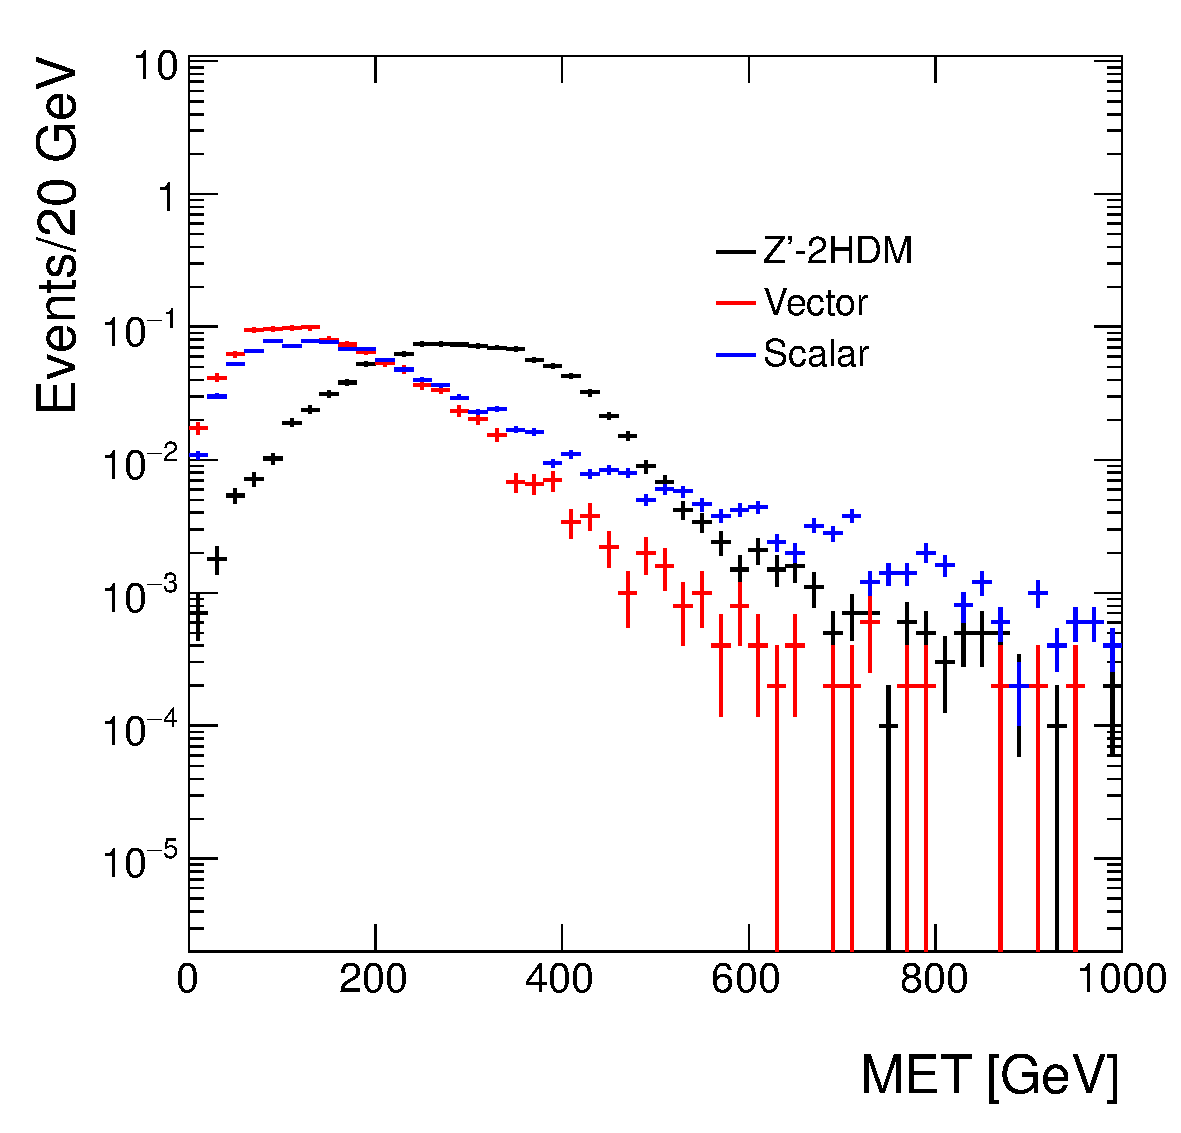
\includegraphics[width=0.60\linewidth]{figures/EW/monoH/models_cmp_MET_et_Log} \label{fig:met_cmp_high}
	}\\
	\subfloat[Low mediator mass]{
		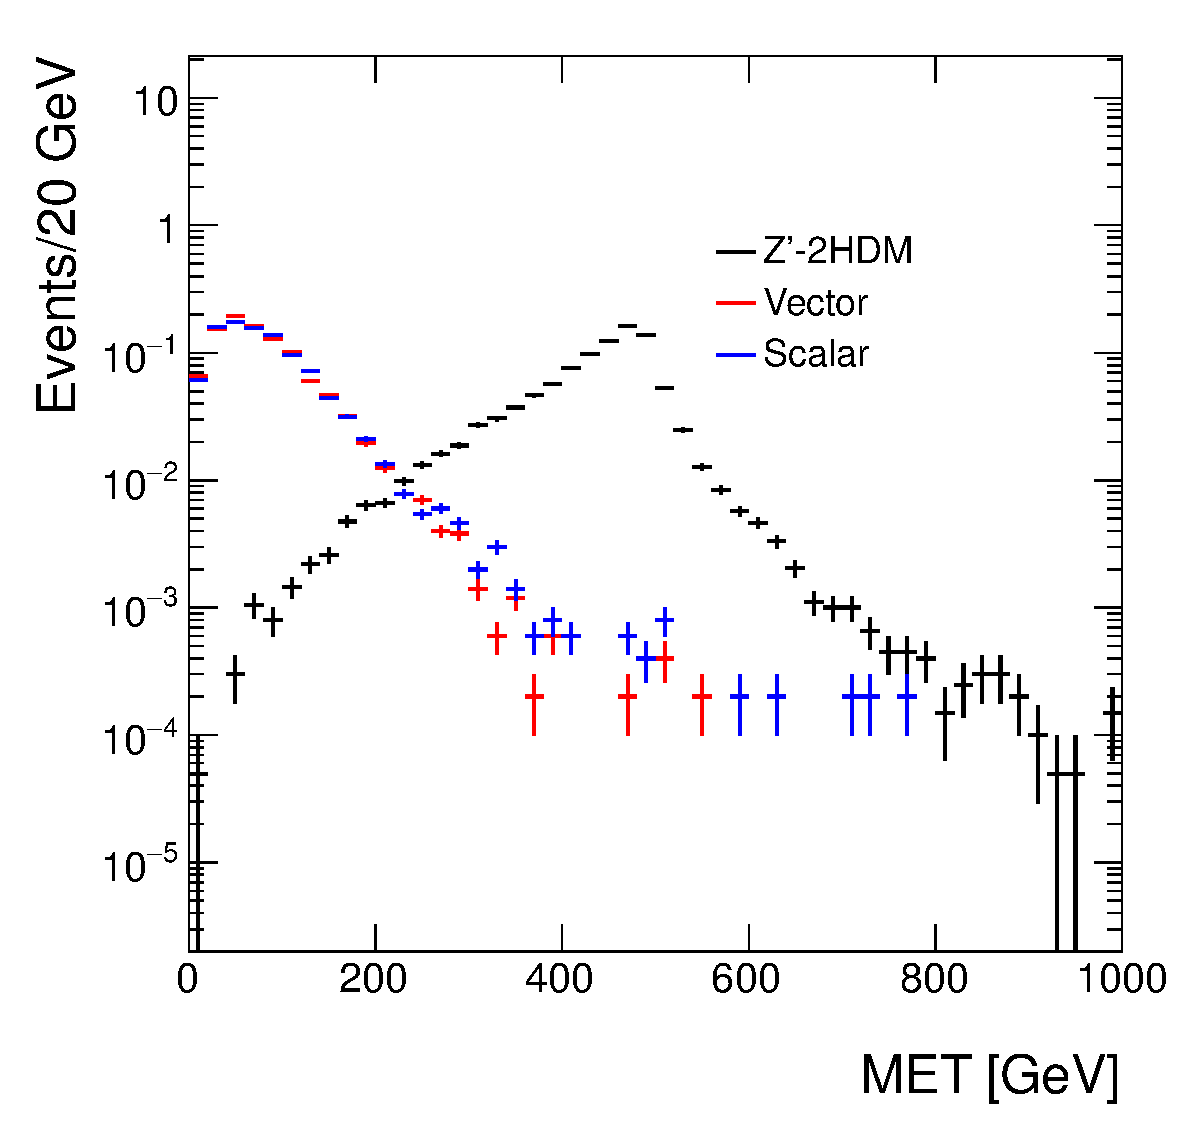
\includegraphics[width=0.60\linewidth]{figures/EW/monoH/models_cmp_low_MET_et_Log} \label{fig:met_cmp_low}
	}
	\caption{Comparison of the missing transverse momentum distributions at generator level in different 
		simplified models leading to a Higgs+\MET signature. The model parameter settings are detailed in the text. The figures in this Section have been obtained using LO UFO models within \madgraph v2.2.3, interfaced to \pythia 8 for the parton shower.  		
		\label{fig:METSimpMonoHiggs}}
\end{figure}

Predictions for this class of models have been so far considered at LO+ Parton Shower (PS), even though they could be extended to NLO+PS in the near future. The studies in this Section
have been performed using a model within \madgraph v5.1.5.12, interfaced to \pythia 6 for the parton shower.  
The implementation details for these models are discussed in Section~\ref{sec:monoHImplementation}.

\subsubsection{\MET+Higgs from a baryonic \Zprime}

The model shown in Fig.~\ref{fig:feyn_prod_monoH} (a)
postulates a new gauge boson \Zprime corresponding to a new $U(1)_B$ baryon 
number symmetry. The stable baryonic states included in this model are the DM candidate particles.
The mass of the \Zprime boson is acquired through a baryonic Higgs $h_B$, which mixes with the 
SM Higgs boson. 

The interactions between the \Zprime, the quarks and the DM are described by 
the following Lagrangian:   

\be \label{ZprimeDM}
	\mathcal{L} =  \gq  \bar q \gamma^\mu q  Z_\mu' +
	 \gDM  \bar\chiDM \gamma^\mu \chiDM Z_\mu' .
\ee

The quark couplings \gq are fixed to be equal to one third of the gauge coupling $g_B$, 
while the DM coupling to the \Zprime are proportional to the baryon number and to the gauge coupling 
($g_{\chiDM} = B g_B$). No leptonic couplings of the \Zprime are allowed, thus evading dilepton constraints. 
After incorporating the mixing of the baryonic and SM Higgs bosons, this model is 
is described by the following Lagrangian term at energies below $m_{\Zprime}$~\footnote{The operator 
	in Eqn.~\ref{U1Beft} is an effective one, to highlight the two main terms. The full dimension-4 simplified
	model is used in the model for event generation.}: 

\be \label{U1Beft}
 \mathcal{L}_{\rm eff} = - \frac{\gq \gDM }{m_{\Zprime}^2} \bar{q} \gamma^\mu q \bar\chiDM \gamma_\mu \chiDM \Big( 1 + \frac{g_{h \Zprime \Zprime} }{m_{\Zprime}^2} h \Big) \, ,
\ee

The first term of this equation
is the standard \modelDMV model in the large $M_{Z^\prime}$ limit.  This term can lead
to a monojet signature, which can be also used to constrain this model.
The second term describes the interaction between the \Zprime and the SM Higgs boson,
via the coupling $g_{h \Zprime \Zprime} = \frac{m_{\Zprime}2 \sin\theta}{v_B}$, where
$\sin\theta$ is the mixing angle between the SM Higgs and the baryonic Higgs $h_B$, and $v_B$ is the
Baryonic Higgs vacuum expectation value. 

%In its most general form, this model can lead to mono-Z signals as well. However, in this case
%there is no $Z-Z'$ mixing from the $h \Zprime \Zprime$ term, since this term arises only
%after $U(1)_B$ is broken. A mixing angle can come from terms involving 
%the field strengths of $Z$ and $Z'$: this is a free parameter, that is set to be small
%in the model considered for mono-Higgs signatures. 

In its most general form, this model can contribute to mono-Z signals due to the \Zprime mixing with the Z or photon. Note that EWSB and $ U(1)_B $ breaking do not lead to this mixing at tree-level. Instead, kinetic mixing occurs between the $ U(1)_Y $ and $ U(1)_B $ gauge bosons due to the gauge invariant term $ F^{\mu\nu}_Y F_{B\mu\nu} $. This mixing is a free parameter which we assume to be small in order to focus on the mono-Higgs signature. Mixing may also occur due to radiative corrections, however we choose to ignore this here as it is model dependent.

The predictions of the model depend upon the two additional
parameters beyond an \schannel simplified model, namely the
mixing angle between baryonic Higgs $h_B$ and the SM-like Higgs boson $\sin\theta$ and the coupling of the mediator to SM-like Higgs boson, $g_{h\Zprime \Zprime}$.
Thus, a full model is specified by:

\be
\left\{\mMed ,\, \mDM ,\, \gDM ,\, \gq ,\, \sin\theta ,\, g_{h\Zprime \Zprime}\right\}.
\ee

\paragraph{Parameter scan} 

The width of the \Zprime mediator is calculated using all possible decays to SM particles (quarks) and to pairs of DM particles if kinematically allowed
as in the \modelDMV model.

The dependence of the missing transverse momentum (\MET) on the model parameters 
is studied by varying the parameters one at a time. The variation of parameters 
other than \mMed and \mDM does not result in significant 
variations of the \MET spectrum, as shown in Figures~\ref{fig:metVectorCoupling}. 
Figure~\ref{fig:metVectorMass} shows that for an on-shell mediator, 
varying \mDM with the other parameters fixed does not affect the \MET distribution, while 
the distribution broadens significantly in the case of an off-shell mediator. 
For this reason, the same grid in \mmed, \mdm as for the vector mediator
of the jet+\MET search (Table~\ref{tab:mDMmMedScan_VA}) is chosen as a starting point. 
The coupling $g_{h\Zprime \Zprime}$, along with \gq and \gDM, are subject to perturbativity bounds:

$$\gq, \gDM < 4\pi $$,

and

$$  g_{h \Zprime \Zprime} < \sqrt{4\pi}m_{\Zprime}\sin\theta$$. 

The value $g_{h \Zprime \Zprime}/m_{\Zprime} = 1$ is chosen as a benchmark value for the generation 
of Monte Carlo samples since it maximizes the cross section (as shown in the following paragraph)
without violating the bounds. The mediator-DM coupling \gDM is fixed to 1, and  
the mediator-quark $g_{q}$ coupling is fixed to 1/3. 
The kinematic distributions do not change as a function of these parameters, so 
results for other values of  $g_{h \Zprime \Zprime}/m_{\Zprime}$, \gDM and \gq can be 
obtained through rescaling by the appropriate cross sections. 

Figs~\ref{fig:VectorHbb_100} and ~\ref{fig:VectorHbb_1000} show the kinematic distributions for the two leading jets
in the $H \to \bar b b$ decay channel, for two values of the mediator mass and varying the DM mass.  

Experimentalists should perform further studies, beyond those studies performed for the forum, 
to estimate the reach of the analysis with respect to all points in the grid and therefore decide 
on a smaller set of grid points to be generated.

\begin{figure}[htpb!]
	\centering
	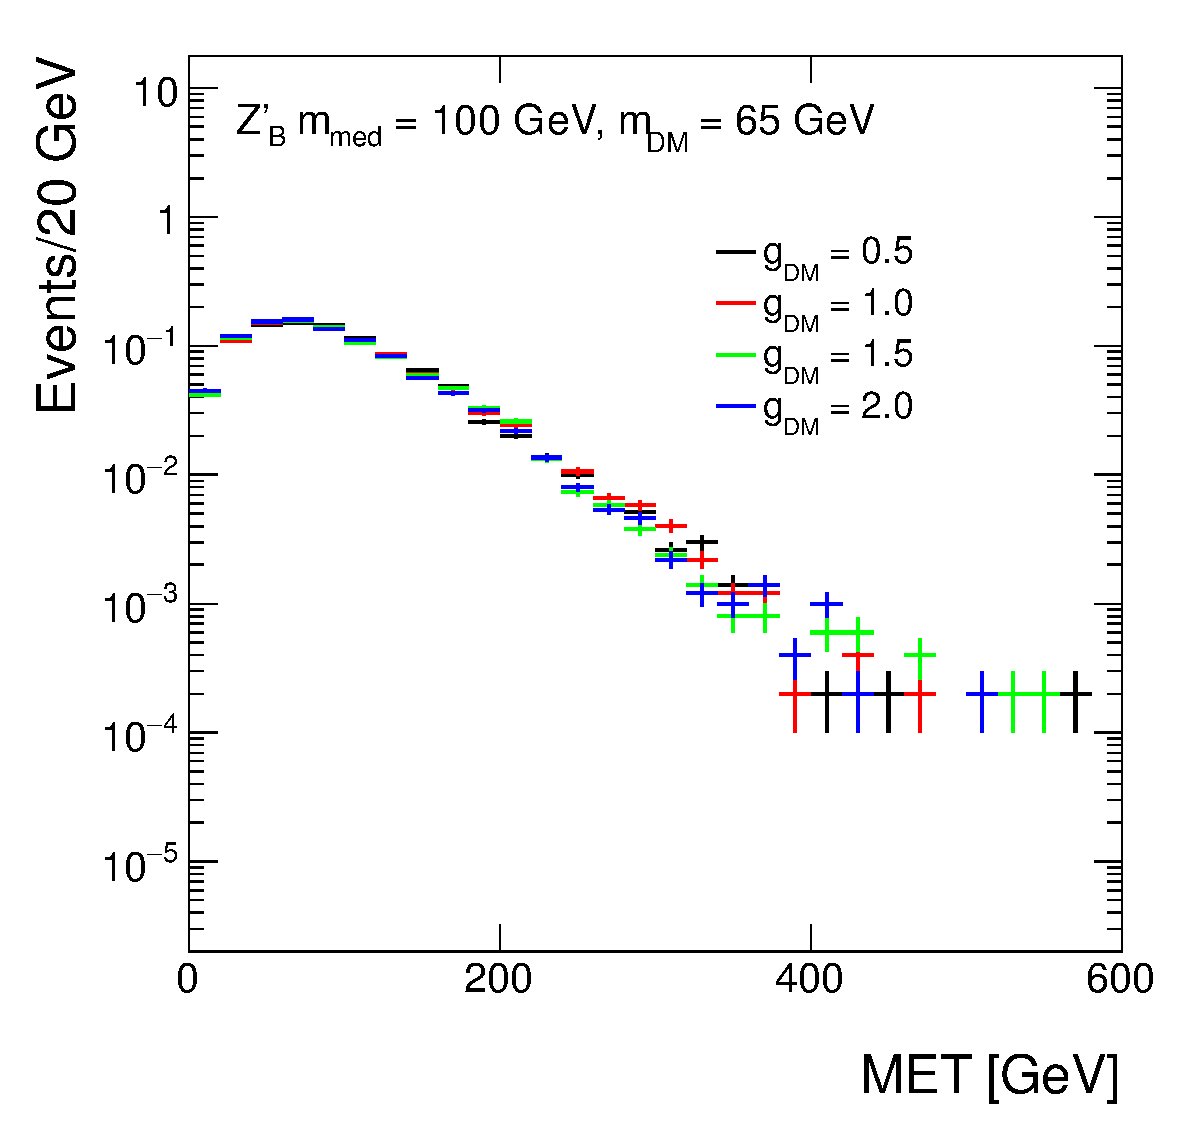
\includegraphics[width=0.60\linewidth]{figures/EW/monoH/z_gdm_MET_et_Log}\\
	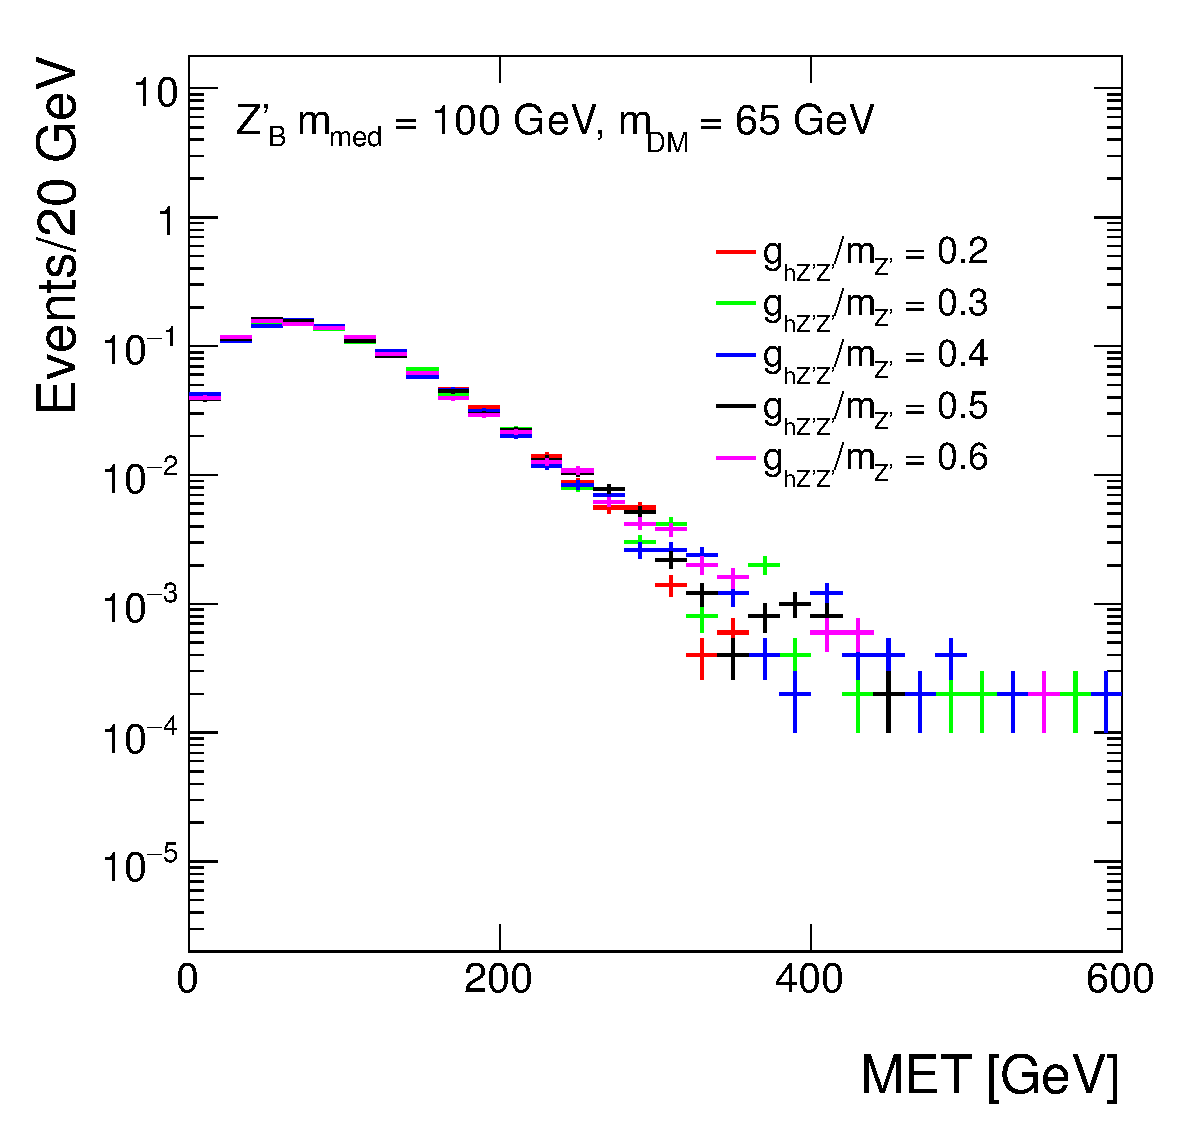
\includegraphics[width=0.60\linewidth]{figures/EW/monoH/z_ratio_MET_et_Log}
	\caption{Missing transverse momentum distributions at generator level in the vector 
		mediator scenario for different values of: the mediator-DM coupling \gDM (left),
		and the coupling between the mediator and the SM-like Higgs boson, scaled by the mediator mass, 
		$g_{h \Zprime \Zprime}/m_{\Zprime}$ (right).
		\label{fig:metVectorCoupling}}
\end{figure}

\begin{figure}[htpb!]
	\centering
	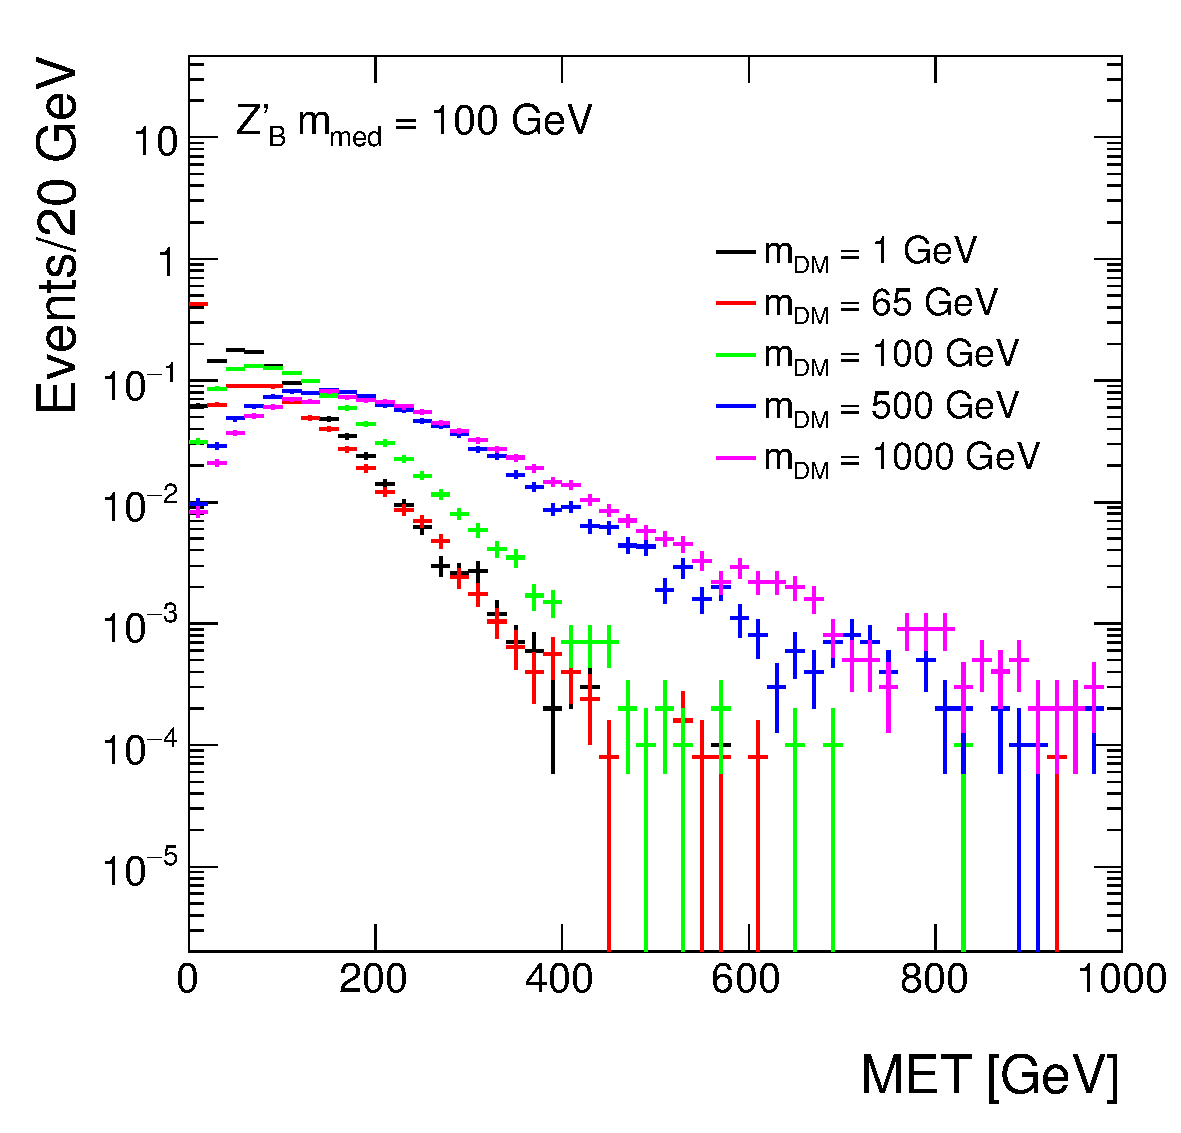
\includegraphics[width=0.60\linewidth]{figures/EW/monoH/zprime_100_MET_et_Log}\\
	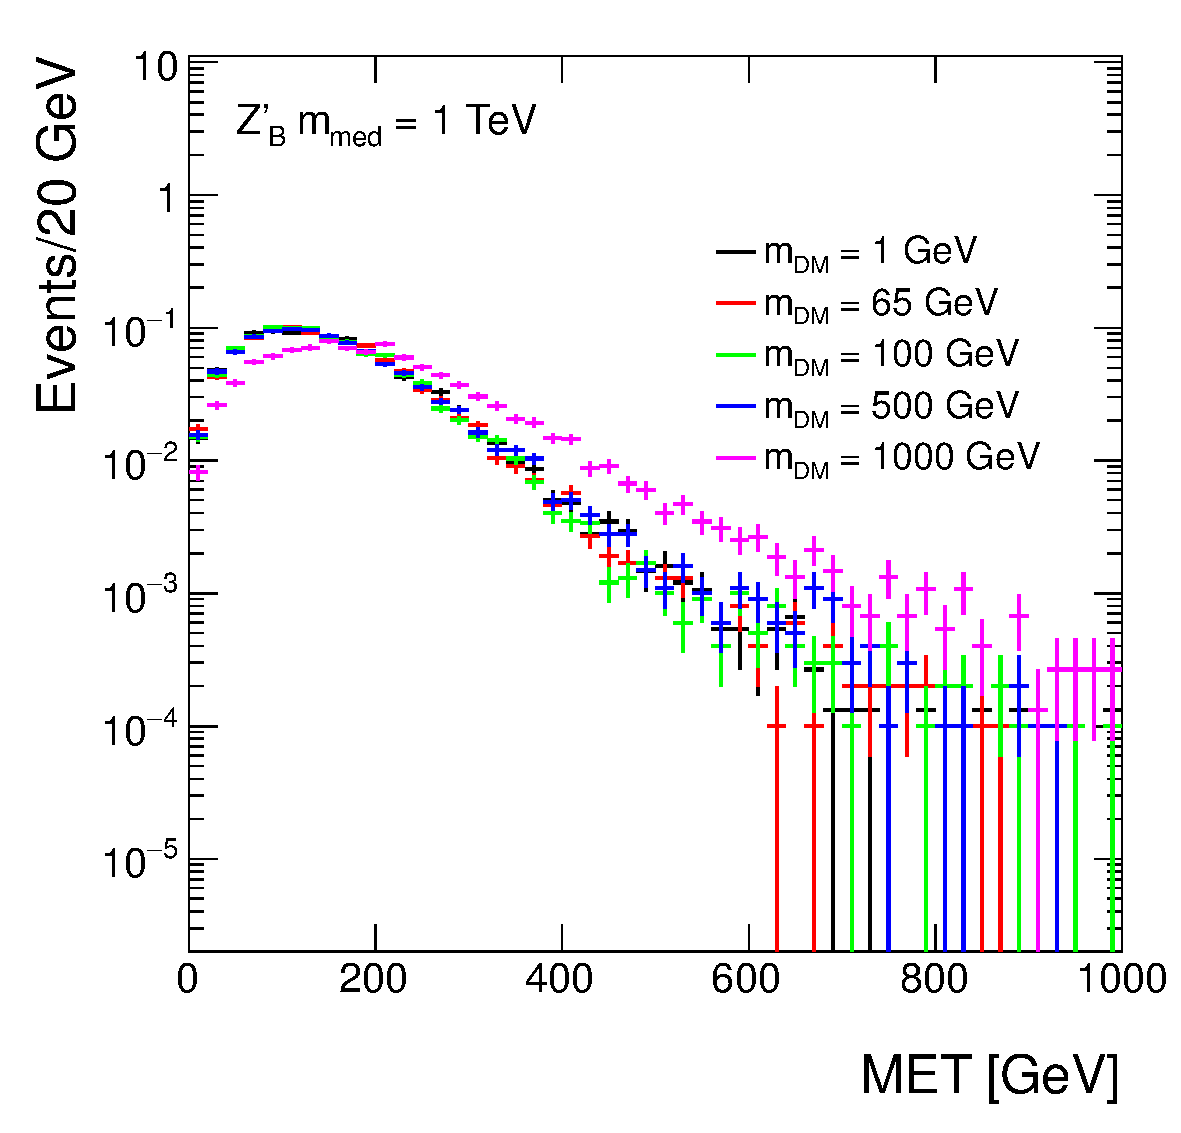
\includegraphics[width=0.60\linewidth]{figures/EW/monoH/zprime_1000_MET_et_Log}
	\caption{Missing transverse momentum distributions at generator level in the vector 
		mediator scenario: for different values of the DM mass \mDM 
		and a mediator mass of \mmed = 100~\gev (left) and \mmed = 1~\tev (right).
		\label{fig:metVectorMass} }
\end{figure}


\begin{figure}[htpb!]
	\centering
	\subfloat[Leading $b-$jet transverse momentum]{
		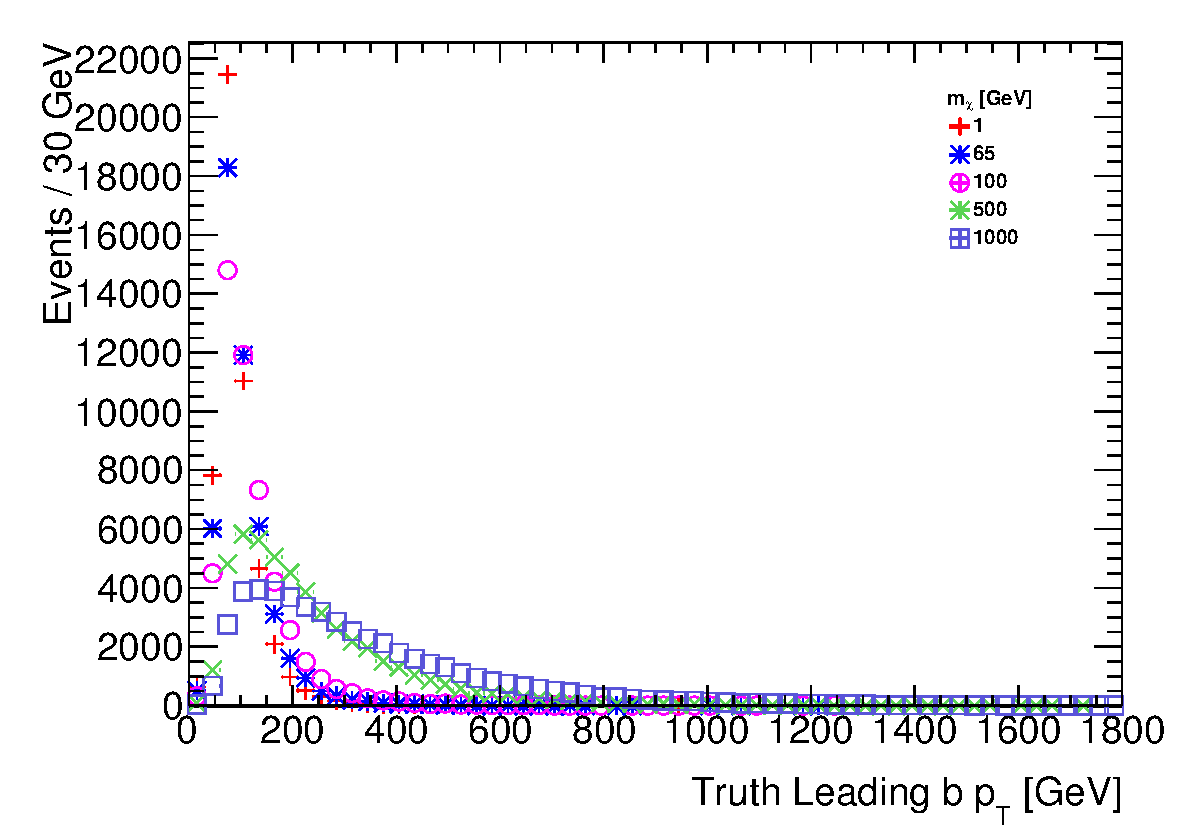
\includegraphics[width=0.60\linewidth]{figures/EW/monoH/zpzp100/truth_leading_b_pt} %\label{fig:met_cmp_high}
	}\hfill
	\subfloat[Leading $b-$jet pseudorapidity]{
		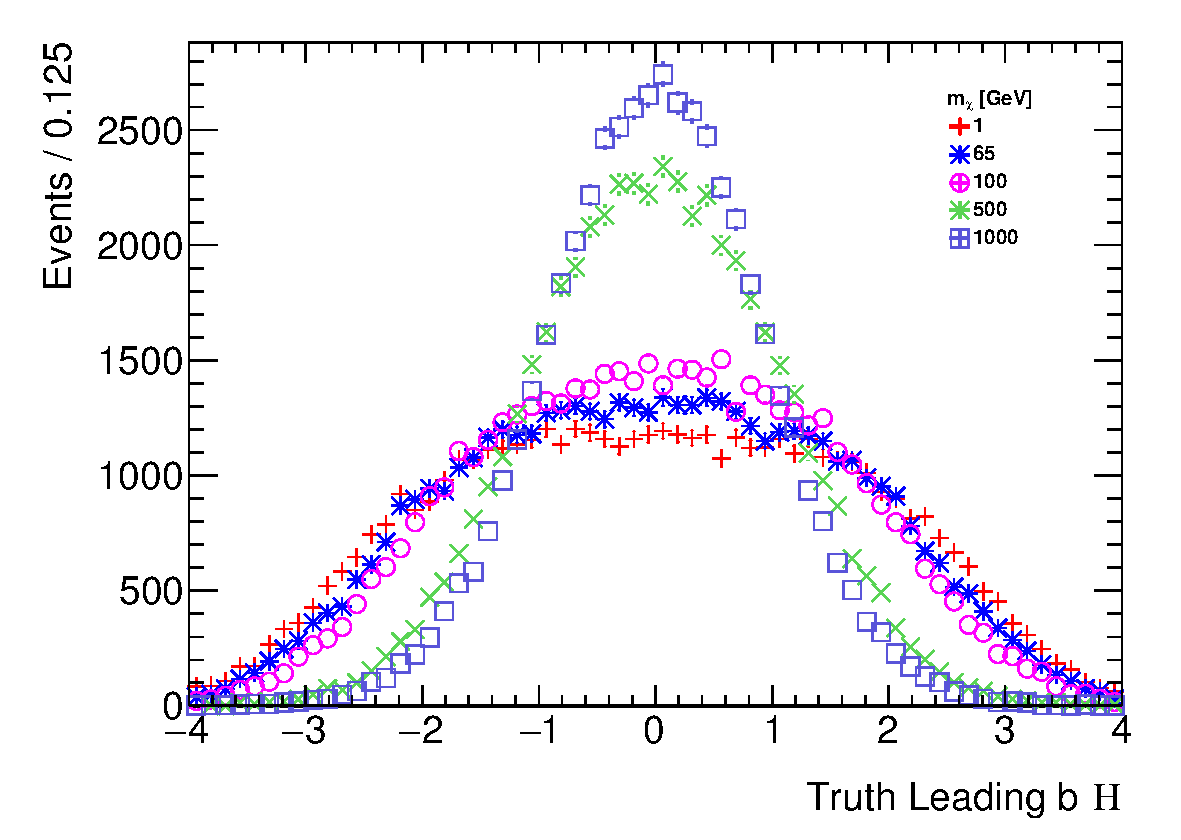
\includegraphics[width=0.60\linewidth]{figures/EW/monoH/zpzp100/truth_leading_b_eta} %\label{fig:met_cmp_low}
	}\hfill
	\subfloat[Angular distance between the two leading $b-$jets]{
		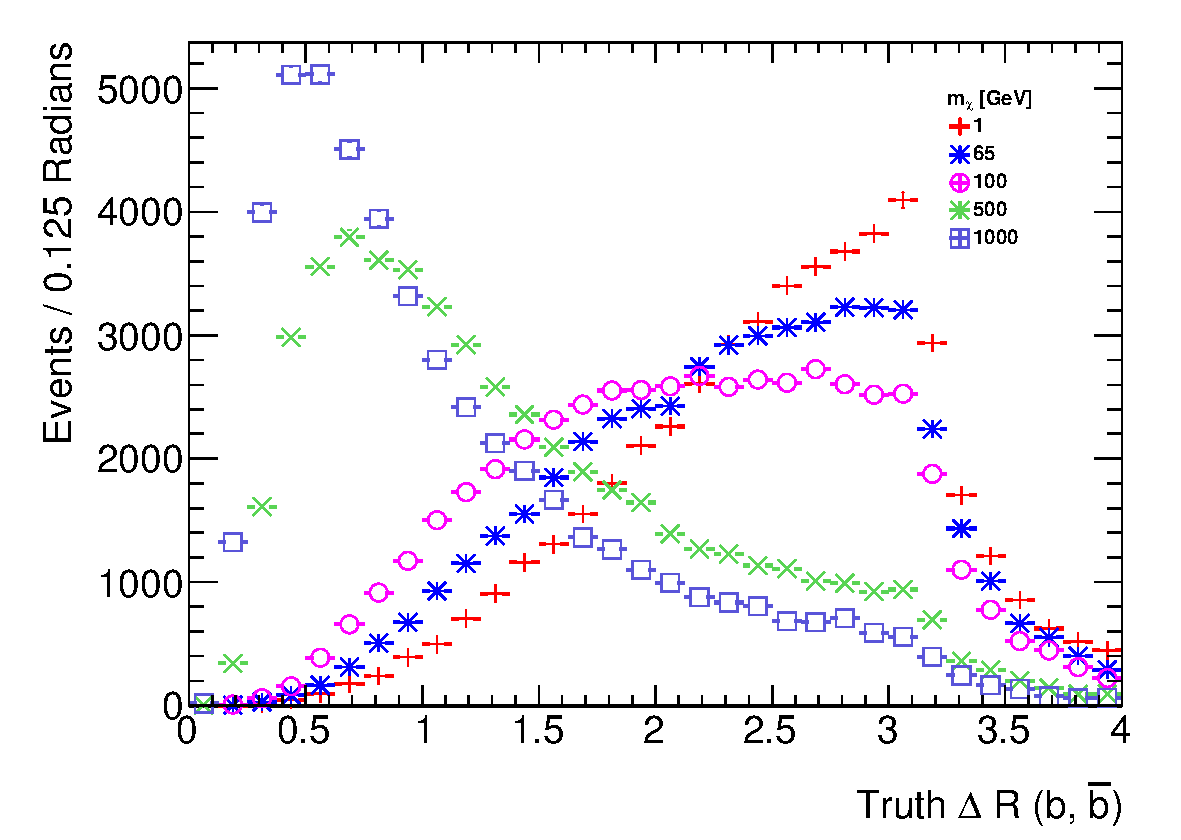
\includegraphics[width=0.60\linewidth]{figures/EW/monoH/zpzp100/truth_bb_deltar} %\label{fig:met_cmp_low}
	}
	\caption{Comparison of the kinematic distributions for the two leading $b-$jets (from the Higgs decay) in the vector \Zprime simplified model, 
		when fixing the \Zprime mass to 100~\gev and varying the DM mass. 
		\label{fig:VectorHbb_100}}
\end{figure}


\begin{figure}[htpb!]
	\centering
	\subfloat[Leading $b-$jet transverse momentum]{
		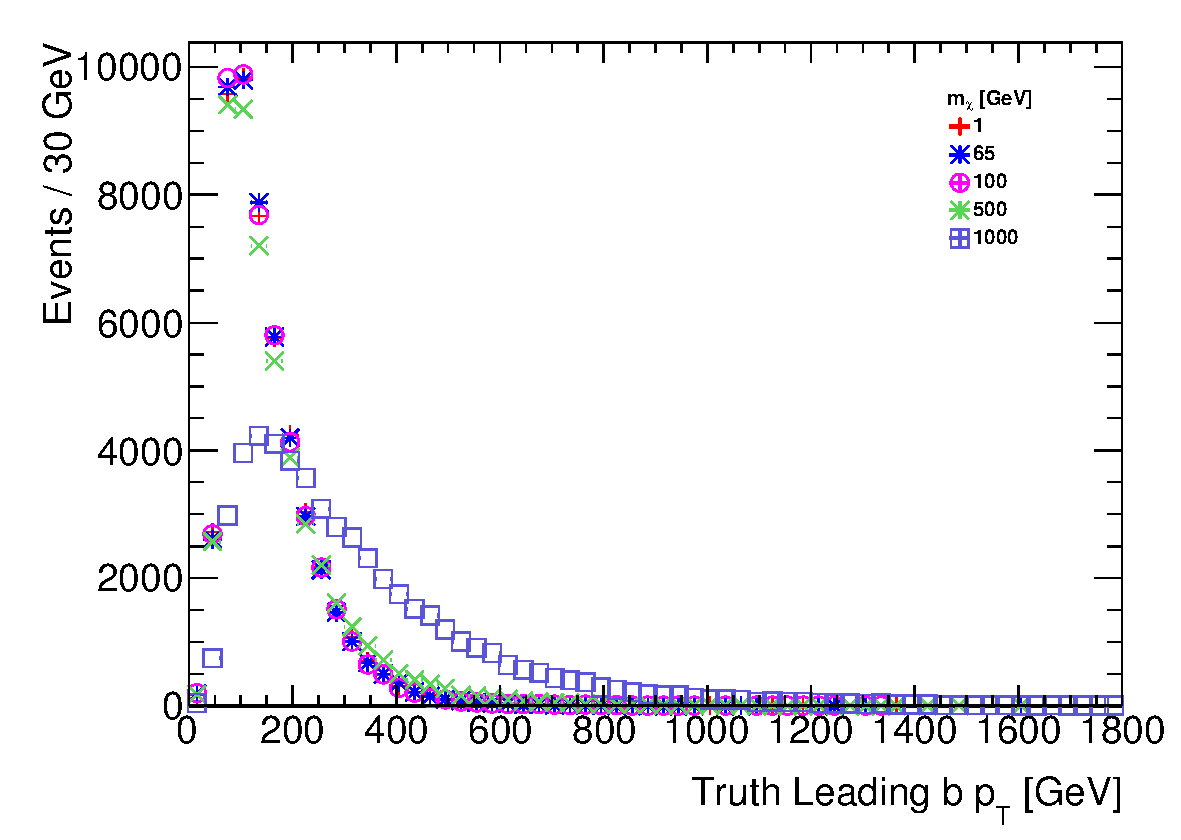
\includegraphics[width=0.60\linewidth]{figures/EW/monoH/zpzp1000/truth_leading_b_pt} %\label{fig:met_cmp_high}
	}\hfill
	\subfloat[Leading $b-$jet pseudorapidity]{
		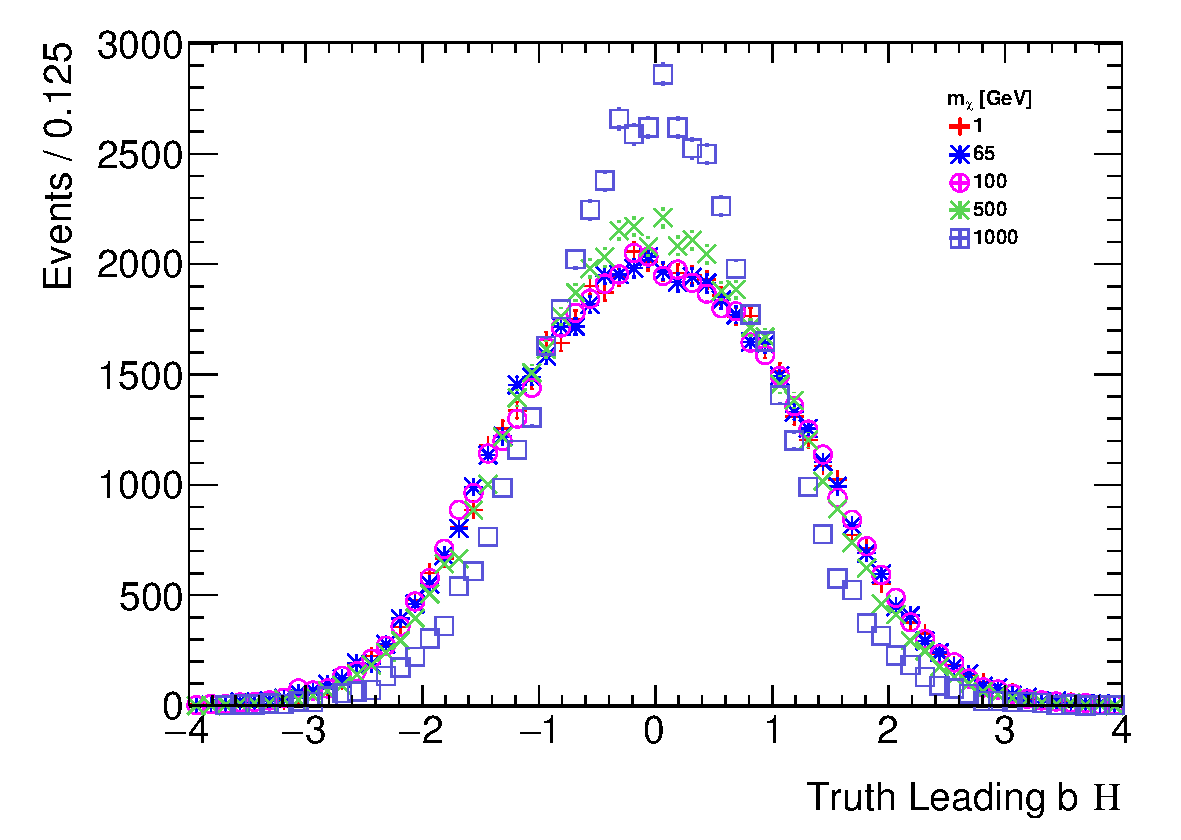
\includegraphics[width=0.60\linewidth]{figures/EW/monoH/zpzp1000/truth_leading_b_eta} %\label{fig:met_cmp_low}
	}\hfill
	\subfloat[\text{Angular separation of the two leading $b$-jets}]{
		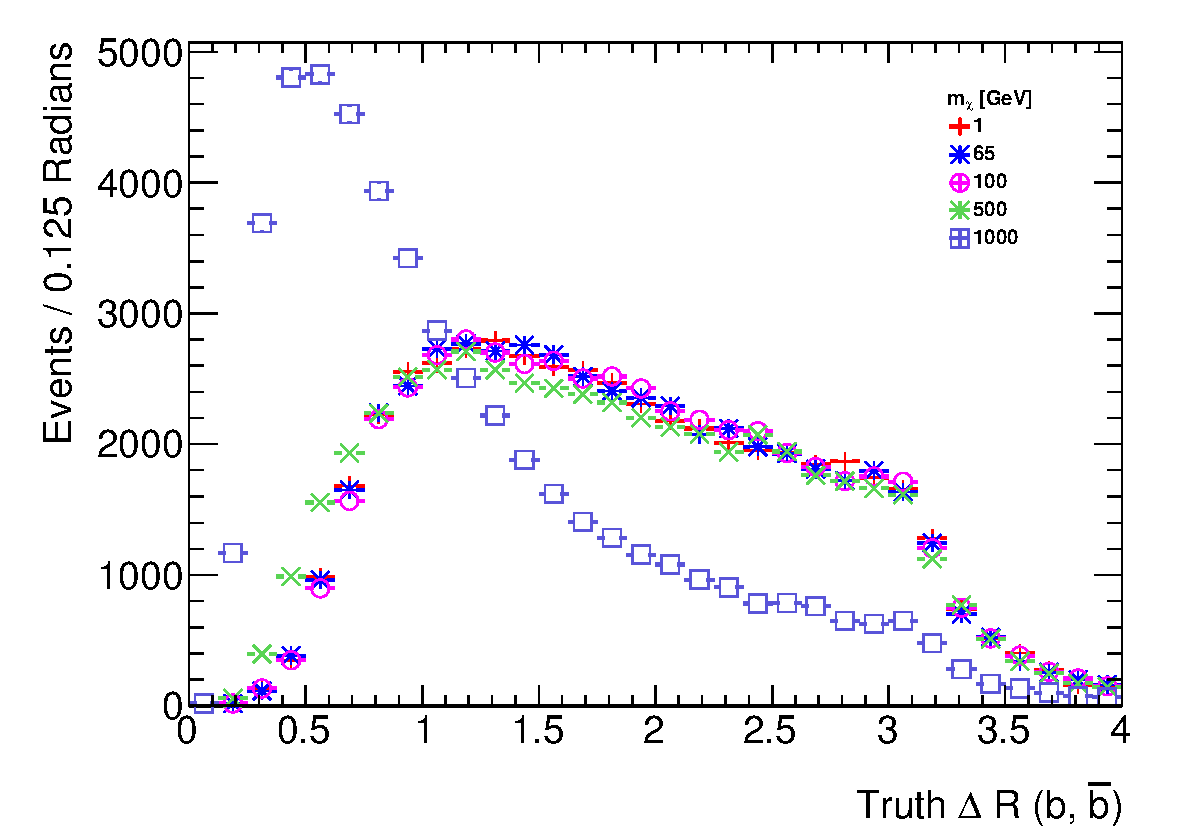
\includegraphics[width=0.60\linewidth]{figures/EW/monoH/zpzp1000/truth_bb_deltar} %\label{fig:met_cmp_low}
	}
	\caption{Comparison of the kinematic distributions for the two leading jets from the Higgs decay in the vector \Zprime simplified model, 
		when fixing the \Zprime mass to 1000~\gev and varying the DM mass. 
		\label{fig:VectorHbb_1000}}
\end{figure}



%%%%\clearpage

\subsubsection{\MET+Higgs from a scalar mediator}

A real scalar singlet $S$ coupling to DM can be introduced as a portal between SM and the dark sector 
through the Higgs field. The most general scalar potential is detailed in Ref.~\cite{O'Connell:2006wi}, 
including terms that break \Ztwo. 
The \Ztwo symmetry, which causes the new scalar to also be a DM candidate, is not covered in this report, but follows Ref.~\cite{Carpenter:2013xra}
introducing an additional coupling to DM that breaks \Ztwo and leads to a new invisible decay of $S$. 
For this reason, no symmetry is broken and no new interactions arise, so there is no dependence on the vacuum
expectation value of $S$: a shift in the field leads to a redefinition of the model couplings. 
The new scalar $S$ mixes with the SM Higgs boson, and couples to DM through a Yukawa term $y_\chiDM$. 
The relevant terms in the scalar potential are:

\begin{align}
&V \supset a |H|^2 S + b |H|^2 S^2 + \lambda_h |H|^4 \notag \\
& \;\;\longrightarrow \tfrac{1}{2} a (h +  v)^2 S + \tfrac{1}{2}b (h +  v)^2 S^2 + \frac{\lambda_h}{4} (h +  v)^4 ,
\label{singlethiggsmix}
\end{align}
where $a,b$ are new physics couplings and $\lambda_h$ is the Higgs quartic coupling.  

The additional Lagrangian terms for this model are: 

\be \label{LintScalar2}
\mathcal{L} \supset - y_\chiDM \bar\chiDM \chiDM (  \cos\theta\:S - \sin\theta\: h ) - \frac{m_q}{v} \bar q q (\cos\theta\: h + \sin\theta\: S )  \,
\ee
where $\theta$ is the mixing angle between the Higgs boson and the new scalar.

Mono-Higgs signals in this second model arise through processes shown in Fig.~\ref{fig:feyn_prod_monoH_S} (a,b), or through 
the radiation of a Higgs boson from the  $t$ quark in the production loop, in Fig.~\ref{fig:feyn_prod_monoH_S} (c). 
The first two processes depend on the $h^2 S$ and $h S^2$ cubic terms in Eq.~\eqref{singlethiggsmix}.  
At leading order in $\sin\theta$, these terms are:

\be
V_{\rm cubic} \approx \frac{\sin\theta}{v} ( 2 m_h^2 + m_S^2) h^2 S  + b \, v \, h \, S^2 + ... , 
\ee
with $a$ and $\lambda_h$ expressed in terms of $\sin\theta$ and $m_h^2$, respectively.  
At leading order of $\sin\theta$, the $h^2 S$ term is fixed once the mass eigenvalues $m_h, m_S$ 
and mixing angle are specified.  The $h\,S^2$ term is not fixed and remains a free parameter of the model, depending on 
the new physics coupling $b$. 

This model also has mono-X signatures through $h/S$ mixing. This model is related to the scalar model discussed in Sec.~\ref{sec:monojet_scalar}
in the case of $m_S \gg m_h$ or $m_h \gg m_S$ and  \mMed equal to the lighter of the two masses, albeit with different mono-Higgs signatures
due to the $h S^2$ vertex. 

\paragraph{Parameter scan}

The model is described by five parameters: 

\begin{enumerate}
	\item the Yukawa coupling of heavy scalar to dark matter, \gDM (also referred to as $y_\chiDM$) 
	\item the mixing angle between heavy scalar and SM-like Higgs boson, $\sin\theta$;
	\item the new physics coupling, $b$;
	\item mass of heavy scalar, $m_{S}$, also termed \mmed;
	\item mass of DM. \mDM;
\end{enumerate}

The mixing angle is constrained from current Higgs data
to satisfy $\cos\theta = 1$ within 10\% and therefore $\sin\theta \lesssim 0.4$. This provides a starting point 
for the parameter scan in this model: we recommend to set $\sin\theta = 0.3$. 

\begin{figure}[hbpt!]
	\begin{center}
		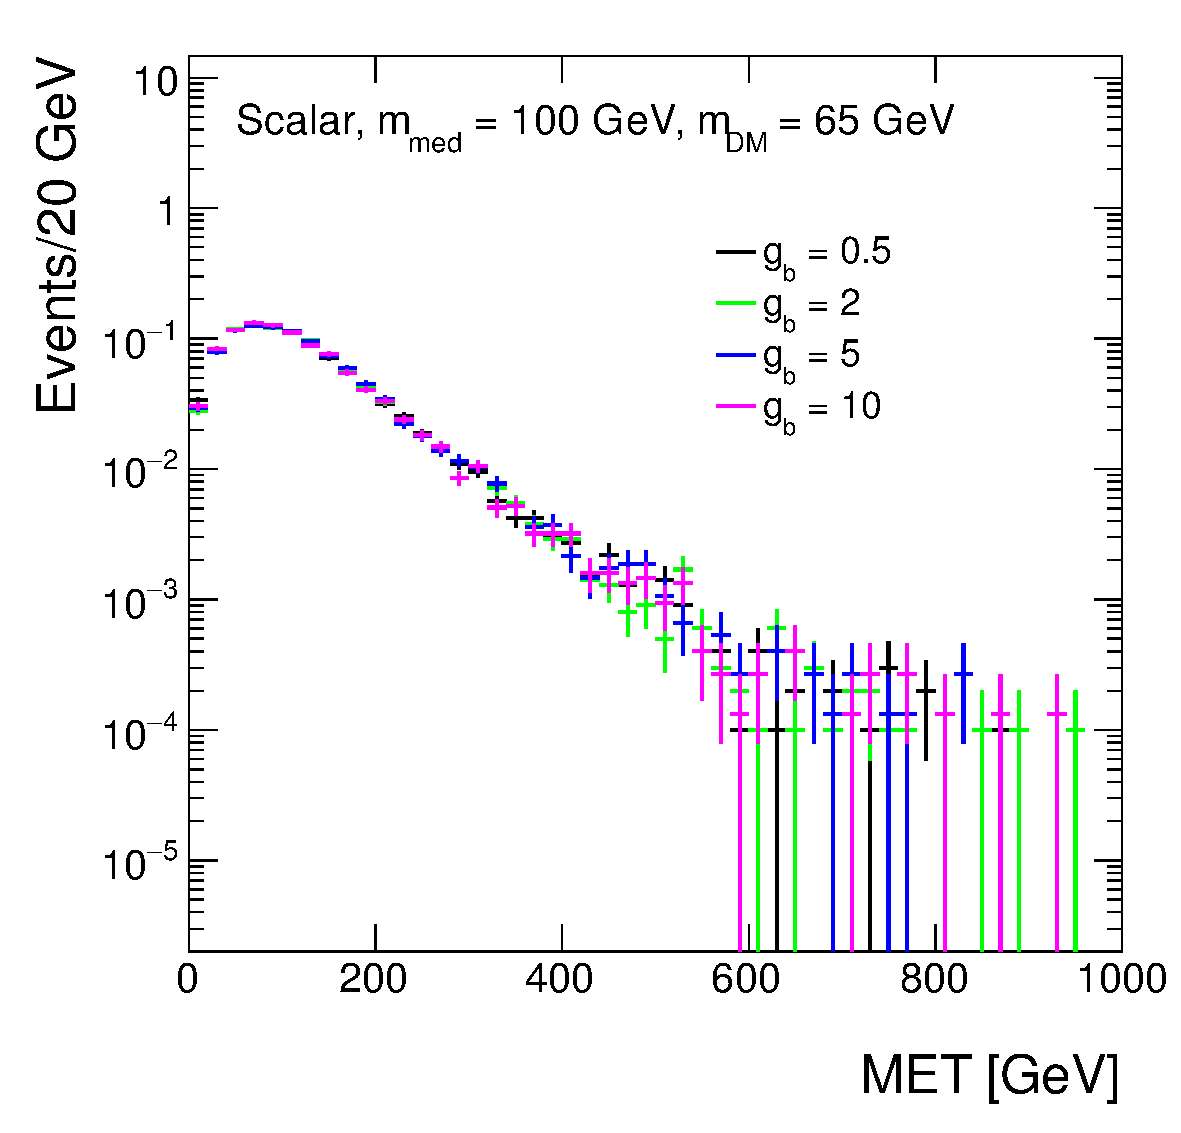
\includegraphics[width=0.75\linewidth]{figures/EW/monoH/s_gb_65_100_04_MET_et_Log}\\
		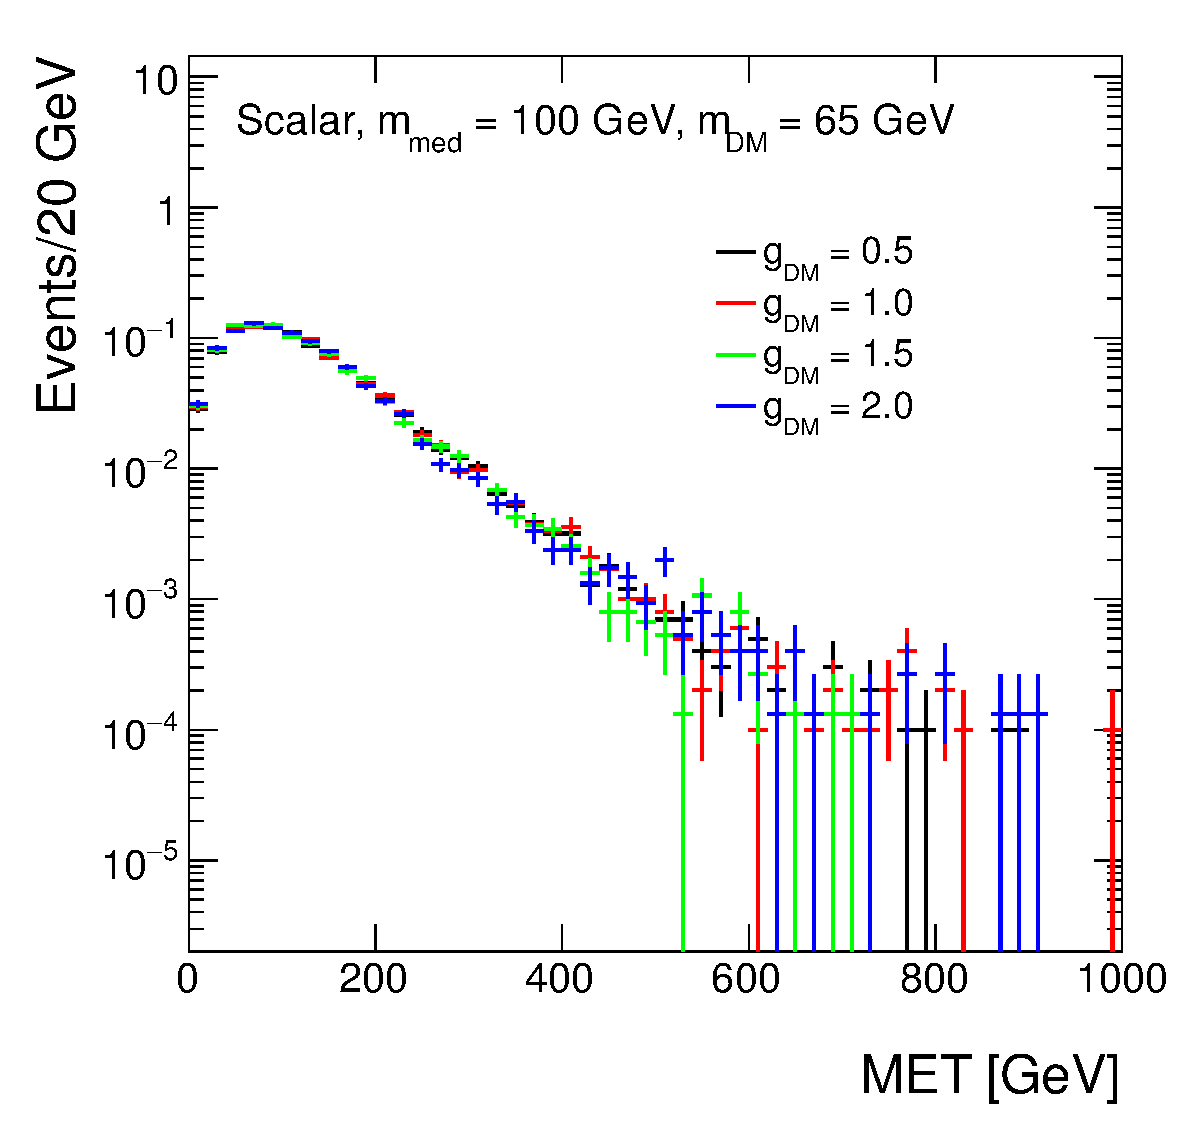
\includegraphics[width=0.75\linewidth]{figures/EW/monoH/s_gdm_MET_et_Log}
		\caption{Missing transverse momentum distributions at generator level in the scalar 
			mediator scenario, for different values of: the new physics coupling $g_b$ (left),
			and the mediator-DM coupling \gDM (right).
			\label{fig:metScalarCoupling}}
	\end{center}
\end{figure}

Figure~\ref{fig:metScalarCoupling2} shows that
the kinematics does not depend on the value of this angle, and results for different values can be obtained via rescaling
the results for this mixing angle according to the relevant cross-section. It can also be observed from Figures~\ref{fig:metScalarMass} and~\ref{fig:metScalarCoupling} 
that the kinematics of this model follows that of the equivalent jet+\MET model: only small changes are observed
in the on-shell region, while the relevant distributions diverge when the mediator is off-shell. 
For this reason, the same grid in \mmed, \mdm as for the scalar mediator
of the jet+\MET search (Table~\ref{tab:mDMmMedScan_SP}) is chosen as a starting point. 
The Yukawa coupling to DM $y_{DM}$ is set to 1, the 
new physics coupling between scalar and SM Higgs $b$ = 3. Results for other values can be obtained via a 
rescaling of the results for these parameters. 



\begin{figure}[hbpt!]
	\begin{center}
		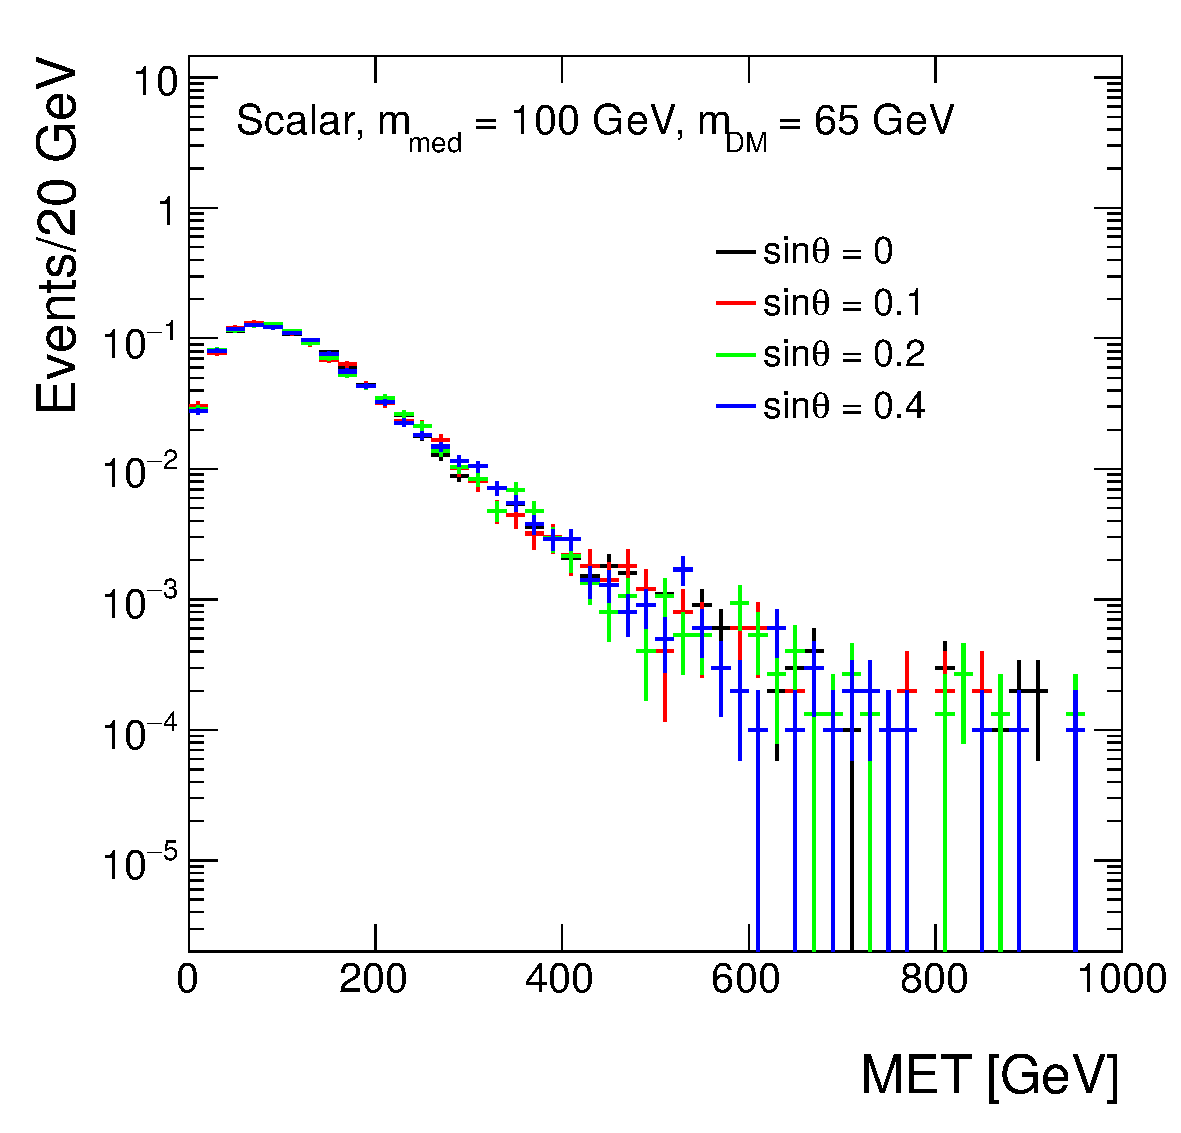
\includegraphics[width=0.75\linewidth]{figures/EW/monoH/s_theta_65_100_2_MET_et_Log}
		\caption{Missing transverse momentum distributions at generator level in the scalar 
			mediator scenario: for different values of the mixing angle $\sin\theta$.
			\label{fig:metScalarCoupling2} }
	\end{center}
\end{figure}

\begin{figure}[hbpt!]
	\begin{center}
		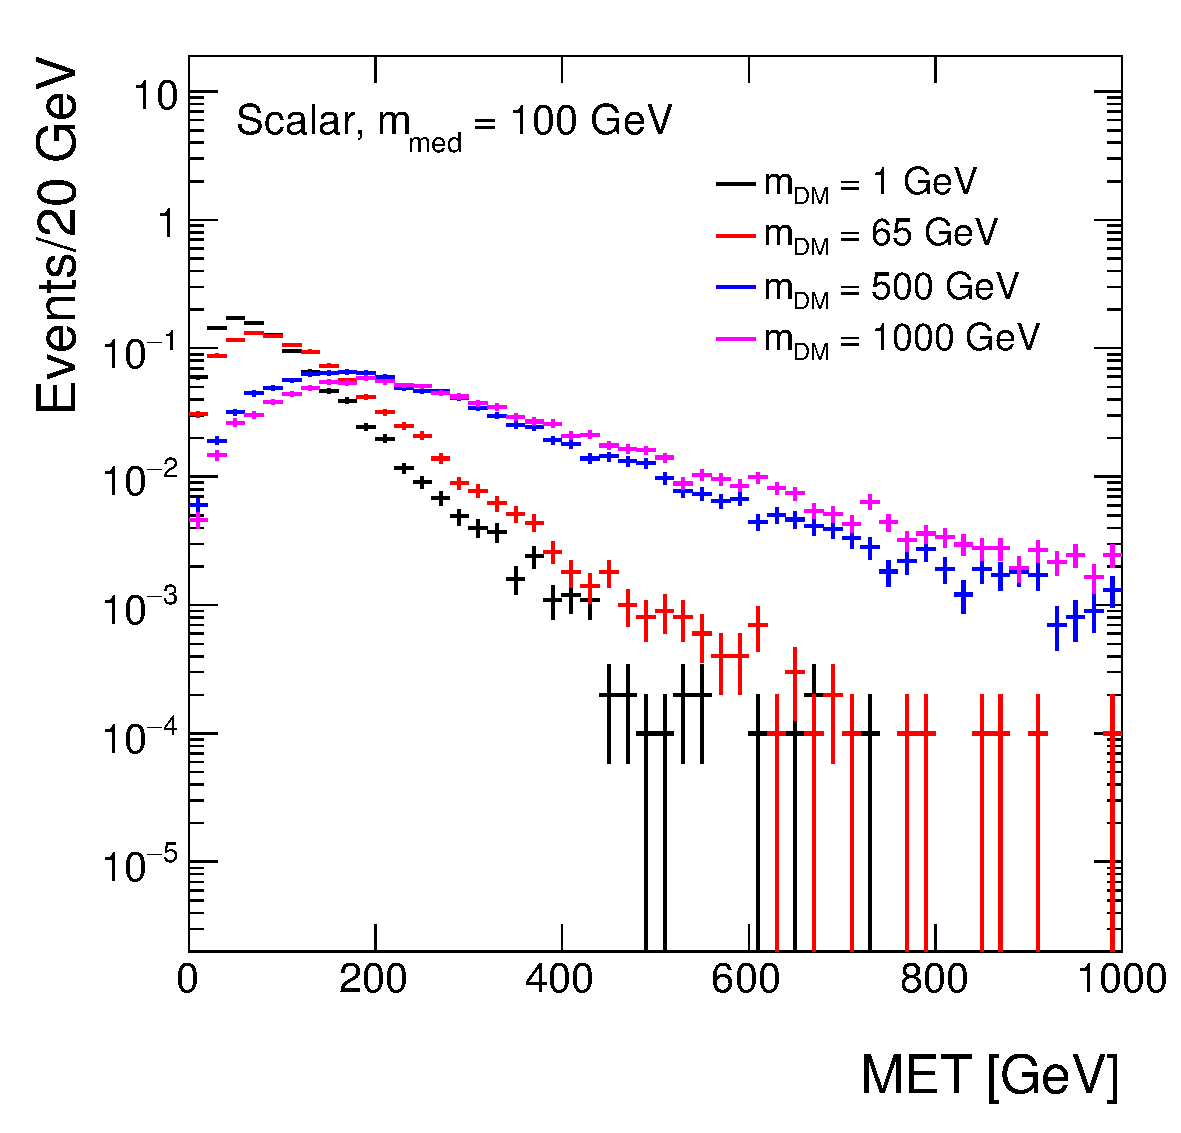
\includegraphics[width=0.75\linewidth]{figures/EW/monoH/scalar_100_MET_et_Log}\\
		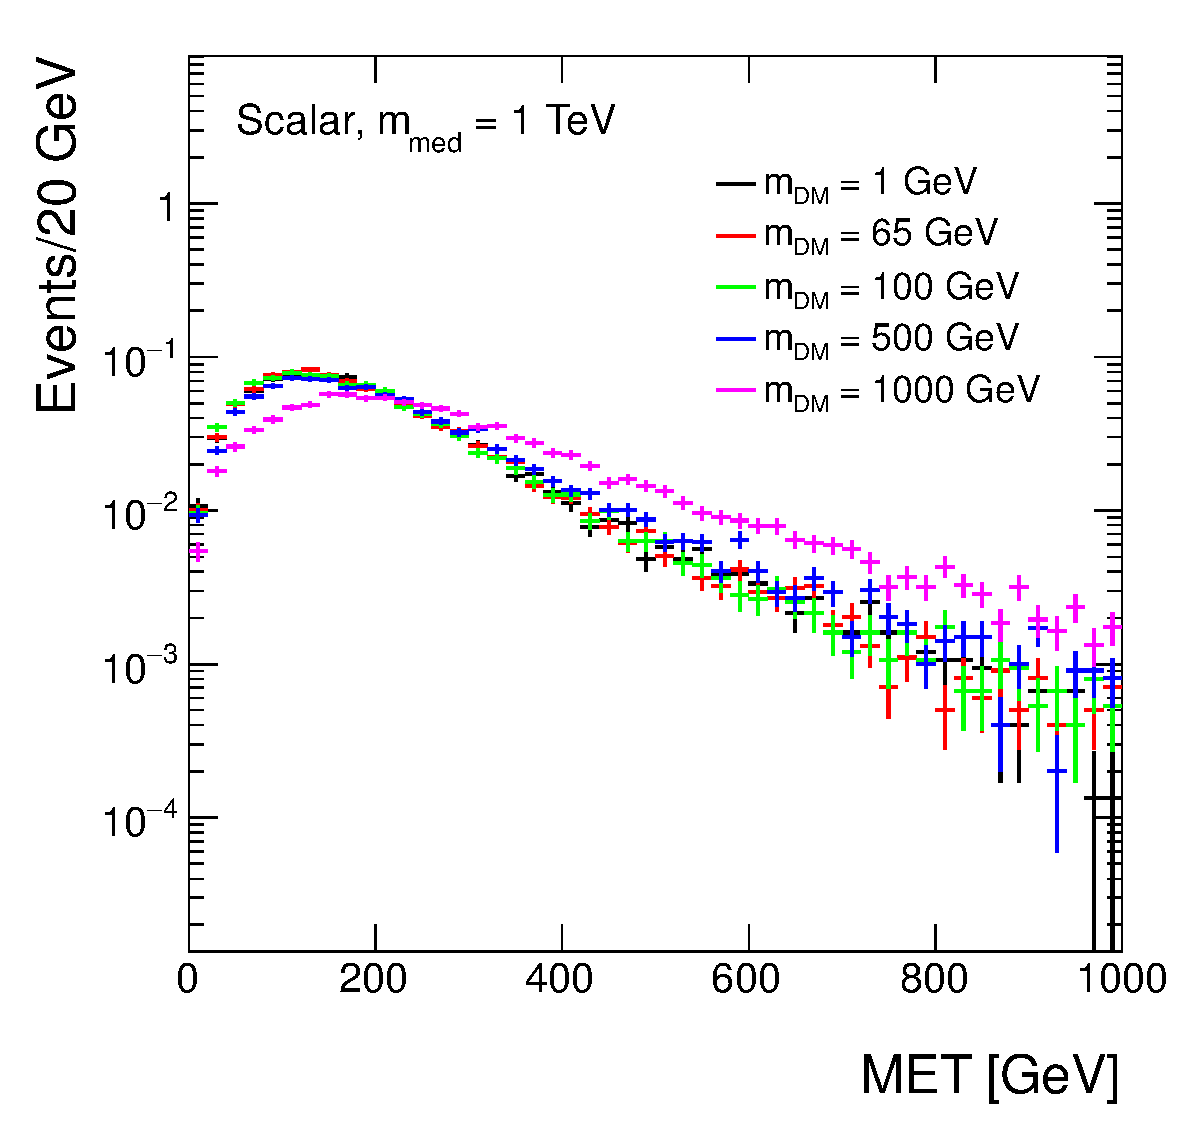
\includegraphics[width=0.75\linewidth]{figures/EW/monoH/scalar_1000_MET_et_Log}
		\caption{Missing transverse momentum distributions at generator level in the scalar 
			mediator scenario: for different values of the DM mass \mDM 
			and a mediator mass of $\mMed = 100~\gev$ (left) and $\mMed = 1~\tev$ (right).
			\label{fig:metScalarMass}}
	\end{center}
\end{figure}

Figs. ~\ref{fig:ScalarHbb_100} and ~\ref{fig:ScalarHbb_1000} show the kinematic distributions for the two leading jets
in the $H \to \bar b b$ decay channel, for two values of the mediator mass and varying the DM mass.  

\begin{figure}[hbpt!]
	\centering
	\subfloat[Leading $b-$jet transverse momentum]{
		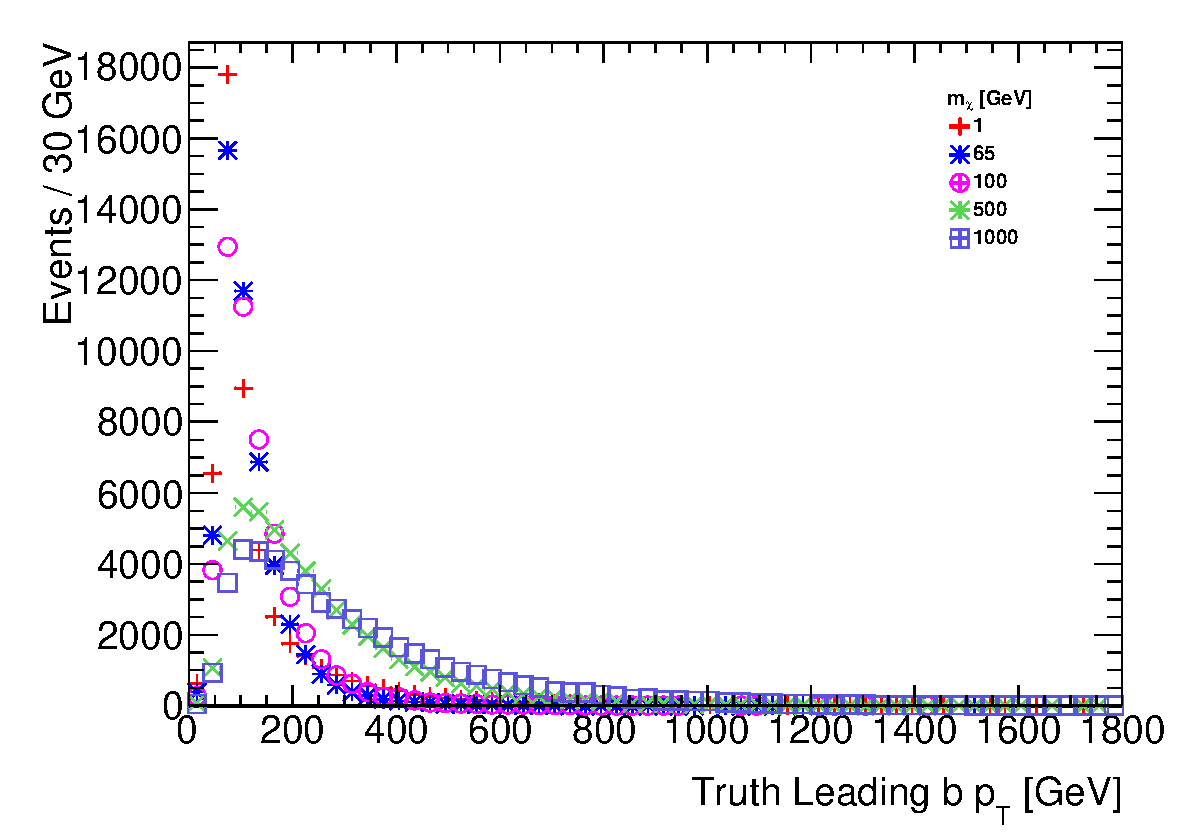
\includegraphics[width=0.60\linewidth]{figures/EW/monoH/scalar100/truth_leading_b_pt} %\label{fig:met_cmp_high}
	}
	\hfill
	\subfloat[Leading $b-$jet pseudorapidity]{
		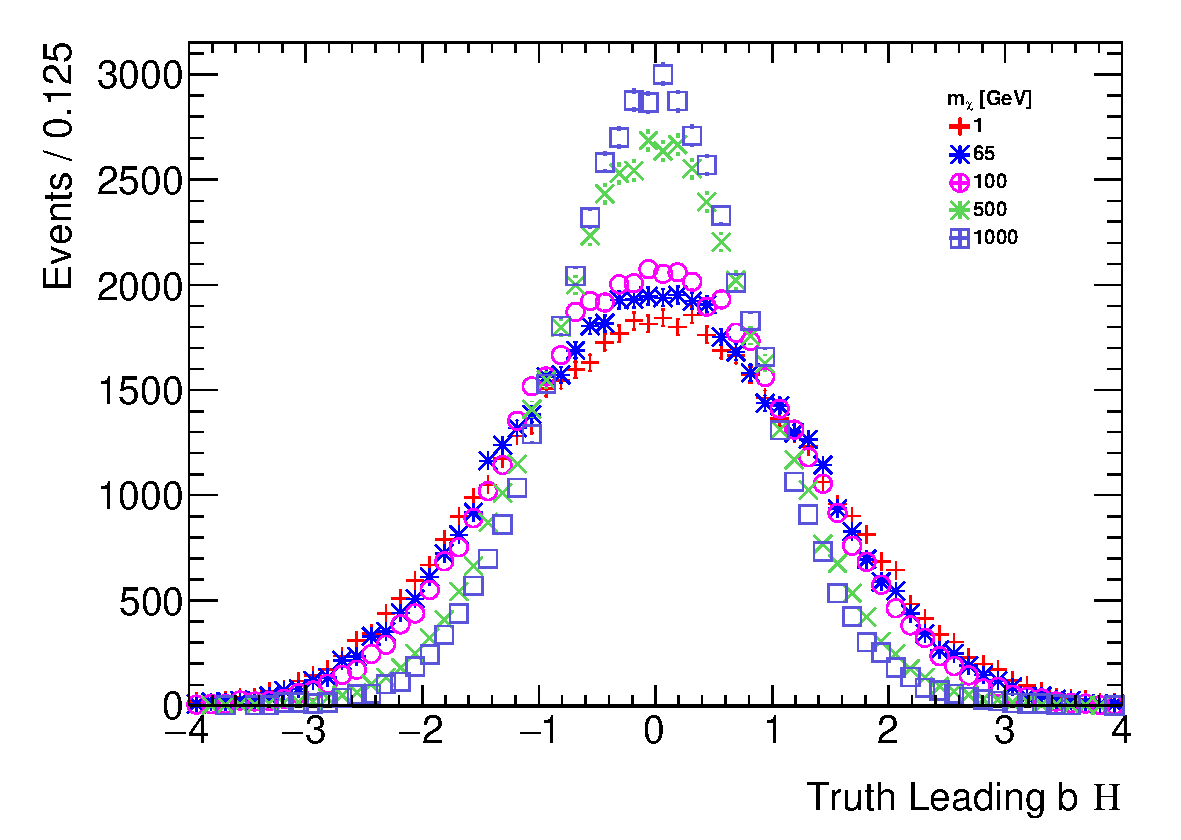
\includegraphics[width=0.60\linewidth]{figures/EW/monoH/scalar100/truth_leading_b_eta} %\label{fig:met_cmp_low}
	}\hfill
	\subfloat[Angular distance between the two leading $b-$jets]{
		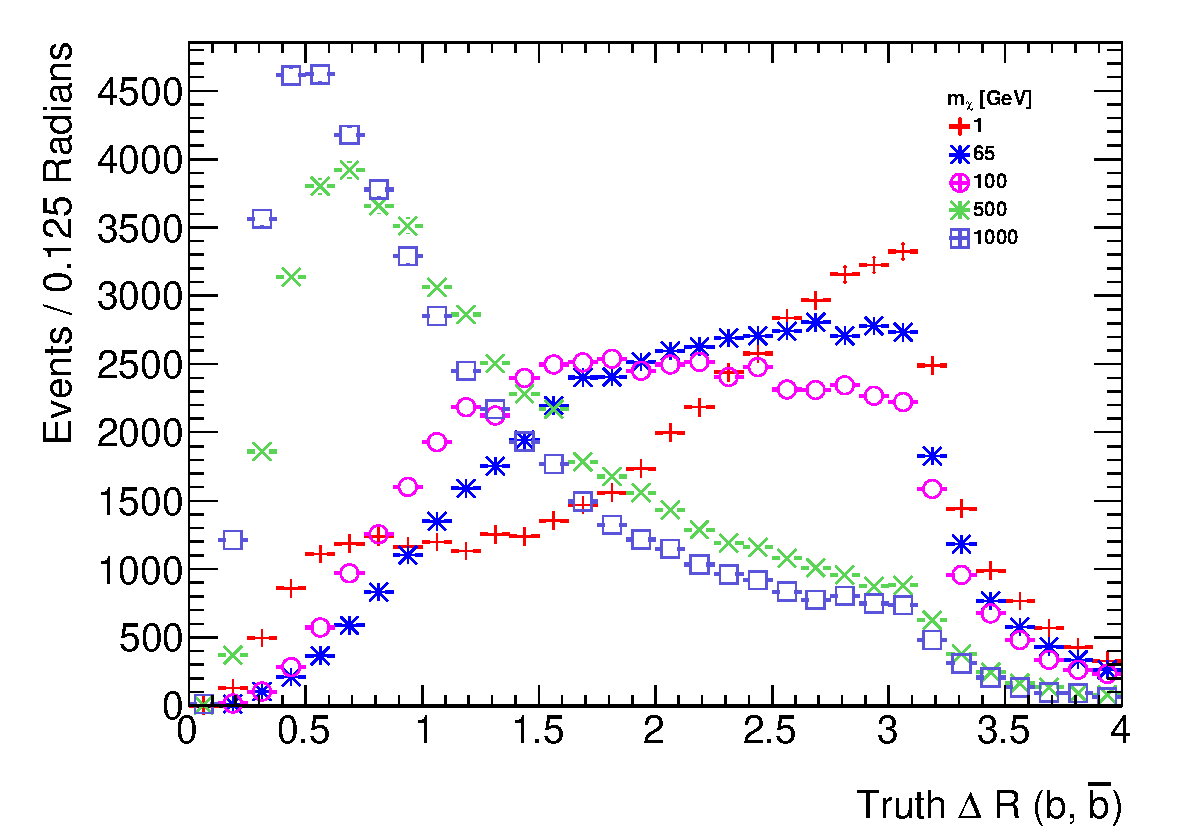
\includegraphics[width=0.60\linewidth]{figures/EW/monoH/scalar100/truth_bb_deltar} %\label{fig:met_cmp_low}
	}

	\caption{Comparison of the kinematic distributions for the two leading jets from the Higgs decay in the scalar simplified model, 
		when fixing the new scalar mass to 100~\gev and varying the DM mass. 
		\label{fig:ScalarHbb_100}}
\end{figure}

\begin{figure}[hbpt!]
	\centering
	\subfloat[Leading $b-$jet transverse momentum]{
		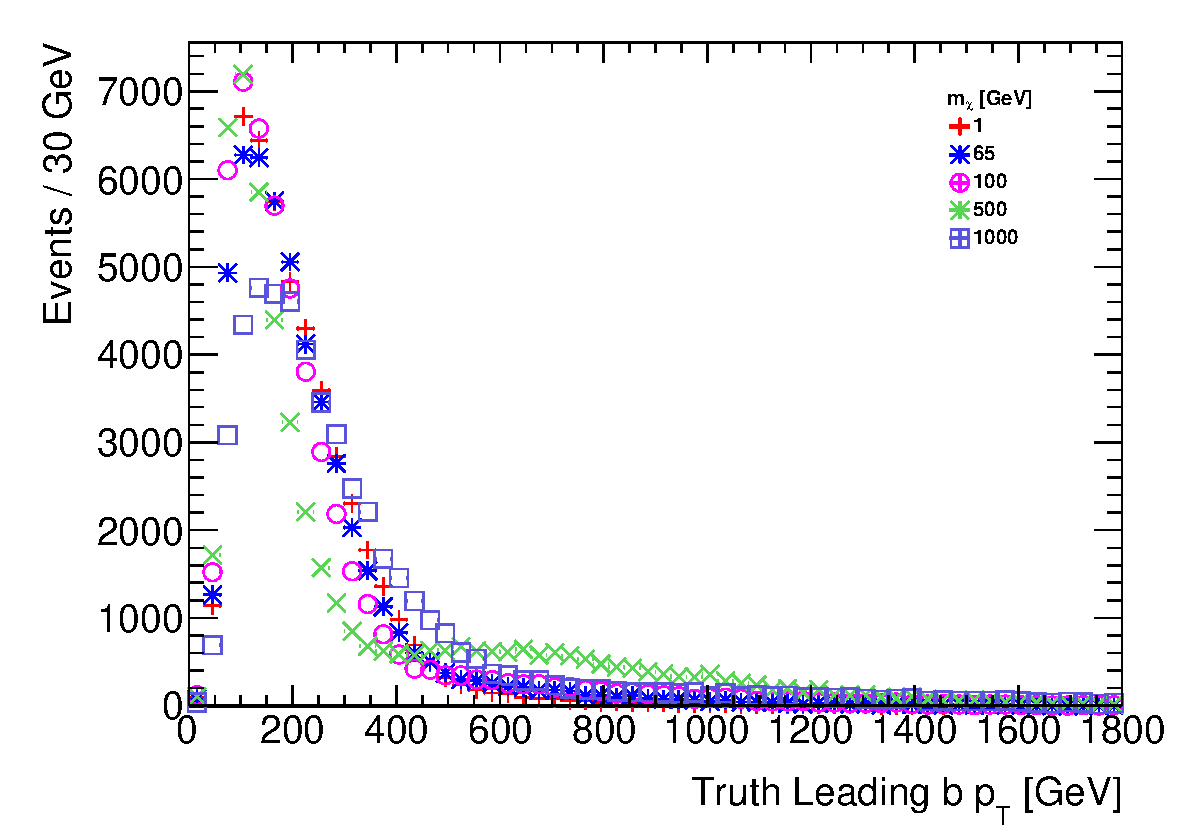
\includegraphics[width=0.60\linewidth]{figures/EW/monoH/scalar1000/truth_leading_b_pt} %\label{fig:met_cmp_high}
	}
	\hfill
	\subfloat[Leading $b-$jet pseudorapidity]{
		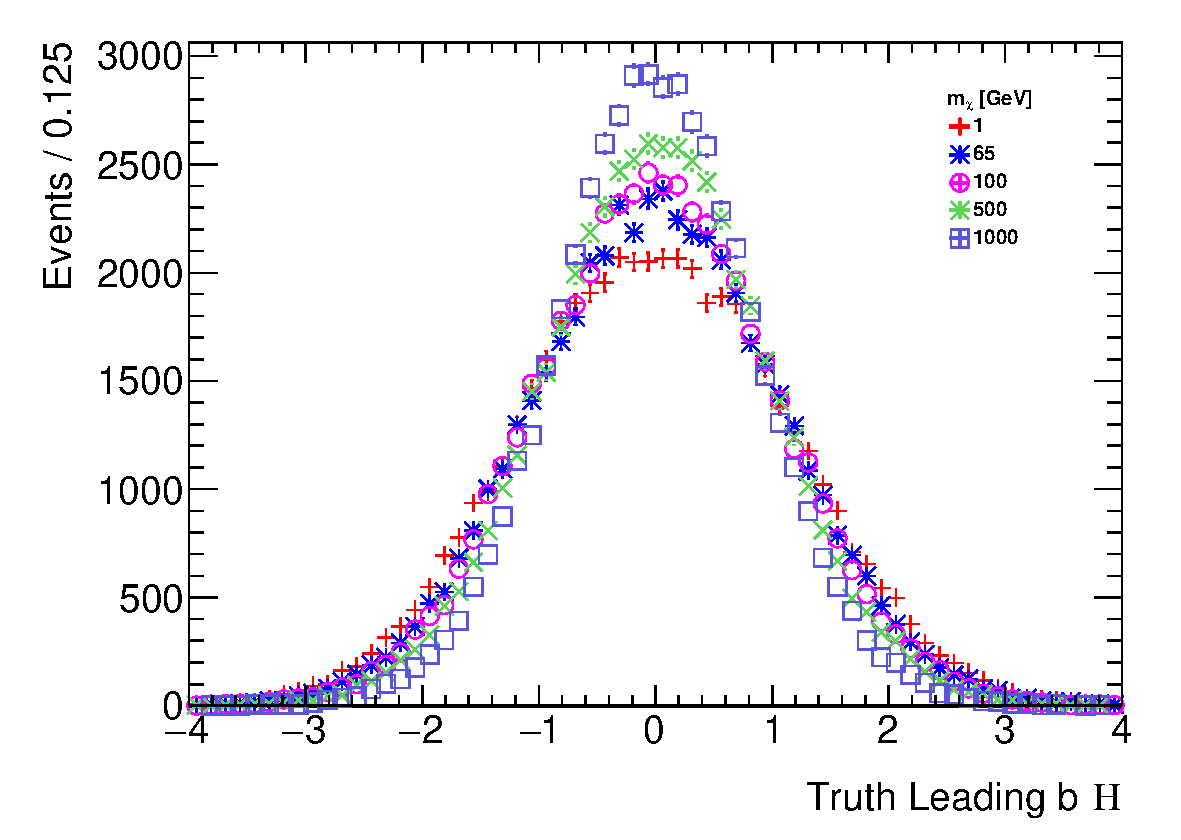
\includegraphics[width=0.60\linewidth]{figures/EW/monoH/scalar1000/truth_leading_b_eta} %\label{fig:met_cmp_low}
	}
	\hfill
	\subfloat[Angular distance between the two leading $b-$jets]{
		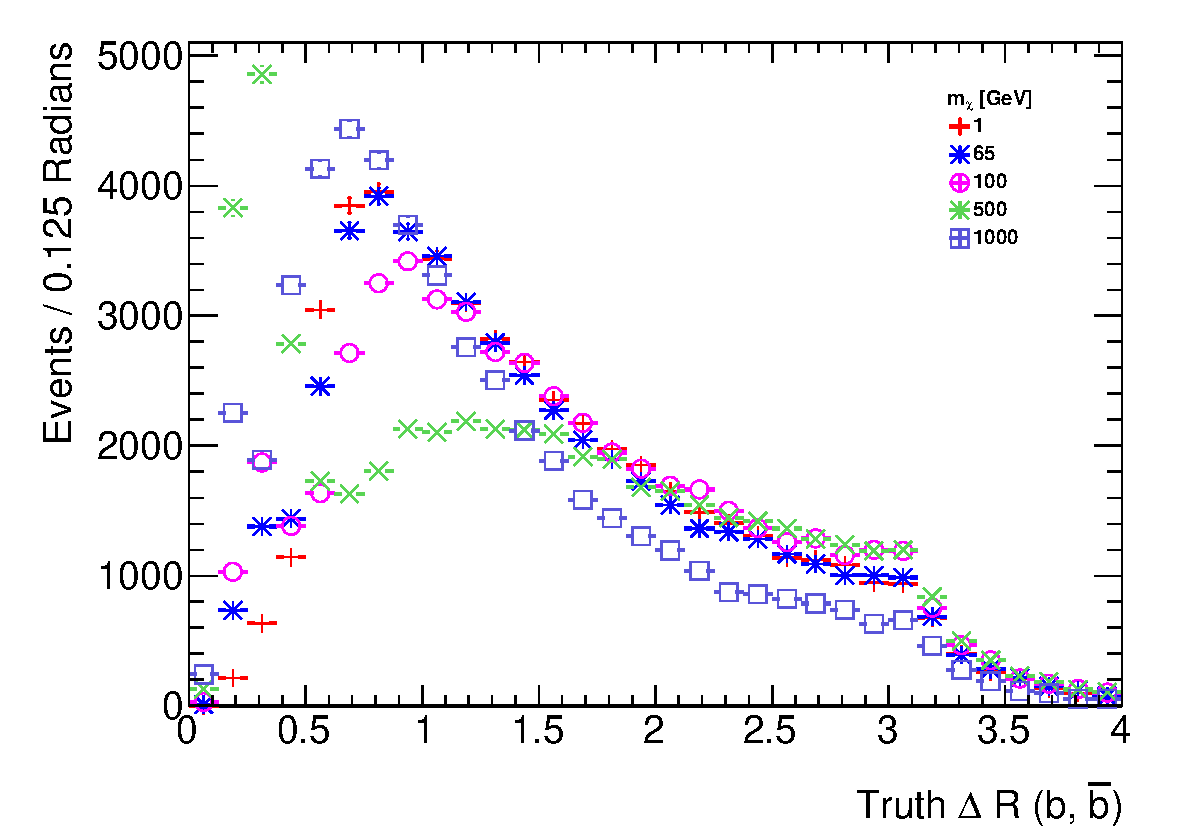
\includegraphics[width=0.60\linewidth]{figures/EW/monoH/scalar1000/truth_bb_deltar} %\label{fig:met_cmp_low}
	}
	\caption{Comparison of the kinematic distributions for the two leading jets from the Higgs decay in the scalar simplified model, 
		when fixing the new scalar mass to 1000~\gev and varying the DM mass. 
		\label{fig:ScalarHbb_1000}}
\end{figure}


%%%
\subsubsection{Higgs+\MET signal from 2HDM model with a \Zprime and a new pseudoscalar}

In this simplified model~\cite{Berlin:2014cfa}, a new \Zprime resonance decays to a Higgs boson $h$ 
plus a heavy pseudoscalar state 
$A^0$ in the 2HDM framework, which in turn decays to a DM pair. This model is 
represented in the diagram in Fig. \ref{fig:feyn_prod_monoH} (b).


The motivation for coupling the DM to the pseudoscalar is that DM coupling to a Higgs or \Zprime boson is generically 
constrained by other signal channels and direct detection.
A reason to consider this model
is that it has different kinematics  due to the on-shell \Zprime production, 
where for heavy \Zprime masses the \MET and $p_T$ spectra are much harder.
This model can satisfy electroweak precision tests and constraints from dijet resonance searches, 
and still give a potentially observable Higgs+\MET signal.
 
The model comprises of two doublets, where $\Phi_u$ couples to up-type quarks and $\Phi_d$ couples to down-type
 quarks and leptons:

 \begin{equation}
 -{\mathcal{L}} \supset  y_u Q \tilde \Phi_u \bar u + y_d Q \Phi_d \bar d + y_e L \Phi_d \bar e  + {\rm h.c.}
 \end{equation}
 
 After electroweak symmetry breaking, the Higgs doublets attain vacuum expectation values $v_u$ and $v_d$, and in unitary gauge the doublets are parametrized as

 \begin{align}
 \Phi_d &= \frac{1}{\sqrt{2}}
 \begin{pmatrix}
 -\sin{\beta} \ H^+ \\ v_d - \sin{\alpha} \ h + \cos{\alpha} \ H - i \sin{\beta} \ A^0
 \end{pmatrix} 
 \quad , \nonumber \\
 \Phi_u &= \frac{1}{\sqrt{2}}
 \begin{pmatrix}
 \cos{\beta} \ H^+ \\ v_u + \cos{\alpha} \ h + \sin{\alpha} \ H + i \cos{\beta} \ A^0
 \end{pmatrix}
 \end{align}
 where $h,H$ are neutral CP-even scalars,
 $H^\pm$ is a charged scalar, and $A^0$ is a neutral CP-odd scalar. 
 In this framework, $\tan{\beta} \equiv v_u/v_d$, and $\alpha$ is the mixing angle that diagonalizes 
 the $h - H$ mass squared matrix. This model also contains an additional scalar singlet $\phi$
 that leads to spontaneous symmetry breaking. 
We take $\alpha = \beta - \pi/2$, in the alignment 
limit where $h$ has SM-like couplings to fermions and 
gauge bosons as per Ref.~\cite{Craig:2013hca}, and $\tan{\beta} \ge 0.3$ 
as implied from the perturbativity of the top Yukawa coupling. 
The Higgs vacuum expectation values lead to $Z-\Zprime$ mass mixing, with a small mixing parameter given by 
 \begin{align}
 \epsilon & \equiv \frac{1}{M_{\Zprime}^2 - M_Z^2} \frac{g g_z}{2 \cos{\theta_w}} ( z_d v_d^2 + z_u v_u^2) \nonumber \\
 & =  \frac{(M_Z^0)^2}{M_{\Zprime}^2 - M_Z^2} \frac{2 g_z \cos \theta_w}{g}  z_u \sin^2 \beta, 
 \label{eq:epsilon}
 \quad
 \end{align}
 where $z_i$ are the $\Zprime$ charges of the two Higgs doublets, and  $g$ and $g_z$ related to the mass-squared
 values in absence of mixing  $(M_Z^0)^2 = g^2(v_d^2+ v_u^2)/(4\cos^2{\theta_w}) $ and
 $(M_{Z'}^0)^2 = g_z^2 ( z_d^2 v_d^2 + z_u^2 v_u^2 + z_\Phi^2
 v_\Phi^2)$. 
    
The production cross section for this model scales as $(g_z)^2$, as the decay width for this process
to leading order in $\epsilon$ (Eq.~\ref{eq:epsilon}) is
\begin{equation}
\Gamma_{\Zprime \to h A^0} =  (g_z \sin \beta \cos \beta)^2 \frac{|p|}{24 \pi} \frac{|p|^2}{M_{\Zprime}^2}.
\end{equation}
where the center of mass momentum for the decay products is
\begin{equation}
|p| = \frac{1}{2 M_{\Zprime}} \sqrt{ (M_{\Zprime}^2 - (m_h + m_{A^0})^2)
(M_{\Zprime}^2 - (m_h - m_{A^0})^2)}.
\end{equation}
The $\Zprime$ can also decay to $Zh$, leading to the same signature if the $Z$ decays invisibly. The partial width for this decay is:
\begin{equation}
\Gamma_{Z' \to hZ}  = (g_z \sin \beta^2)^2 \frac{|p|}{24 \pi} \left( \frac{ |p|^2 }{M_{Z'}^2} + 3 \frac{M_Z^2}{M_{Z'}^2} \right).
\end{equation} We recommend to generate these two decays separately and combine them at a later stage. 

%\frac{1}{2 M_{\Zprime}} \lambda^{1/2}(M_{\Zprime}^2,m_h^2, m_{A^0}^2)$, and
%$\lambda$ is the K\"{a}llen triangle function\footnote{\vskip -2.5\baselineskip%\begin{align*}\lambda(c_1,c_2,c_3) \equiv&\;c_1^2 + c_2^2 + c_3^2\\ 
%						&- 2(c_1 c_2 + c_2 c_3 + c_3 c_1)\end{align*}}.
   
%  Diagonalizing the gauge
% boson mass matrix, the tree-level masses of the $Z$ and \Zprime bosons are given by
% \begin{align}
% M_Z^2 &\approx ( M_{Z}^0)^2  - \epsilon^2 \left[( M_{\Zprime}^0)^2 - ( M_{Z}^0)^2 \right] \nonumber \\
% M_{\Zprime}^2 &\approx ( M_{\Zprime}^0)^2 + \epsilon^2 \left[( M_{\Zprime}^0)^2 - ( M_{Z}^0)^2 \right]
% \quad ,
% \label{eq:Zpmasses}
% \end{align}
% where $(M_Z^0)^2 = g^2(v_d^2+ v_u^2)/(4\cos^2{\theta_w}) $ and
% $(M_{\Zprime}^0)^2 = g_z^2 ( z_d^2 v_d^2 + z_u^2 v_u^2 + z_\phi^2
% v_\phi^2)$ are the mass-squared values in the absence of mixing. The
% result above is accurate to order $\epsilon^2$, where $\epsilon$ is
% a small mixing parameter given by
% \begin{align}
% \epsilon & \equiv \frac{1}{M_{\Zprime}^2 - M_Z^2} \frac{g g_z}{2 \cos{\theta_w}} ( z_d v_d^2 + z_u v_u^2) \nonumber \\
% & =  \frac{(M_Z^0)^2}{M_{\Zprime}^2 - M_Z^2} \frac{2 g_z \cos \theta_w}{g}  z_u \sin^2 \beta.
% \label{eq:epsilon}
% \quad
% \end{align}
 
\paragraph{Parameter scan}
 
 The model is described by five parameters:
 \begin{itemize}
 	\item the pseudoscalar mass $M_{A^0}$,
 	\item the DM mass \mDM,
 	\item the \Zprime mass, $M_{\Zprime}$,
        \item $\tan{\beta} (\equiv v_u/v_d)$,
 	\item the \Zprime coupling strength $g_z$. 
 \end{itemize}
 
 To study the signal production and kinematic dependencies on these parameters, 
 we produced signal samples varying each of the five parameters through 
 \madgraph for the matrix element, \pythiaEight for the parton shower, and DELPHES\cite{deFavereau:2013fsa}  for a parameterized detector-level simulation.
 
 As seen in Fig.~\ref{fig:DMH_tanbeta}, variations of $\tan{\beta}$ does not lead to any kinematic 
 difference and the production cross section simply scales as a function of $\tan{\beta}$. Hence 
we recommend to fix $\tan{\beta}$ to unity in the signal generation. 


\begin{figure}[htpb!]
\centering
\subfloat[\MET distribution]{
	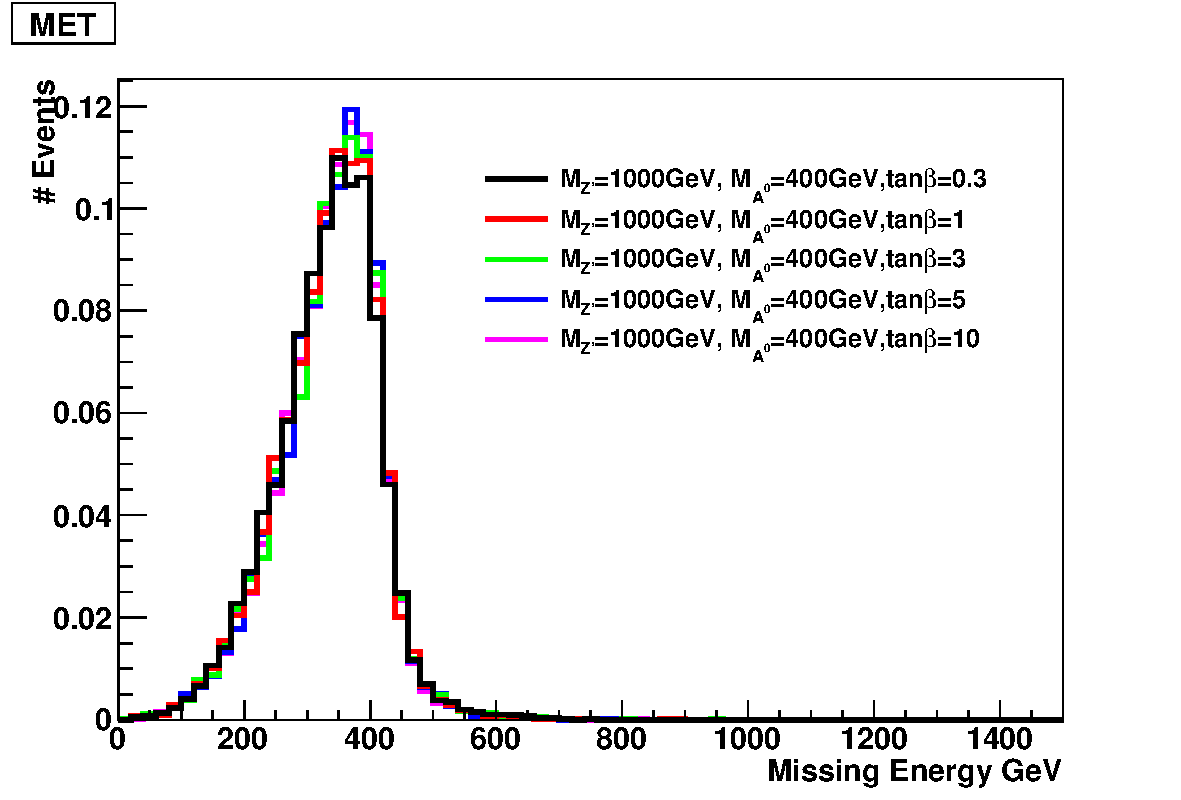
\includegraphics[width=0.60\linewidth]{figures/EW/monoH/2hdm/hxx_zp1000dm10gz01_met}
}
\hfill
\subfloat[$\Delta\phi$ distance between the two $b-$ jets]{
	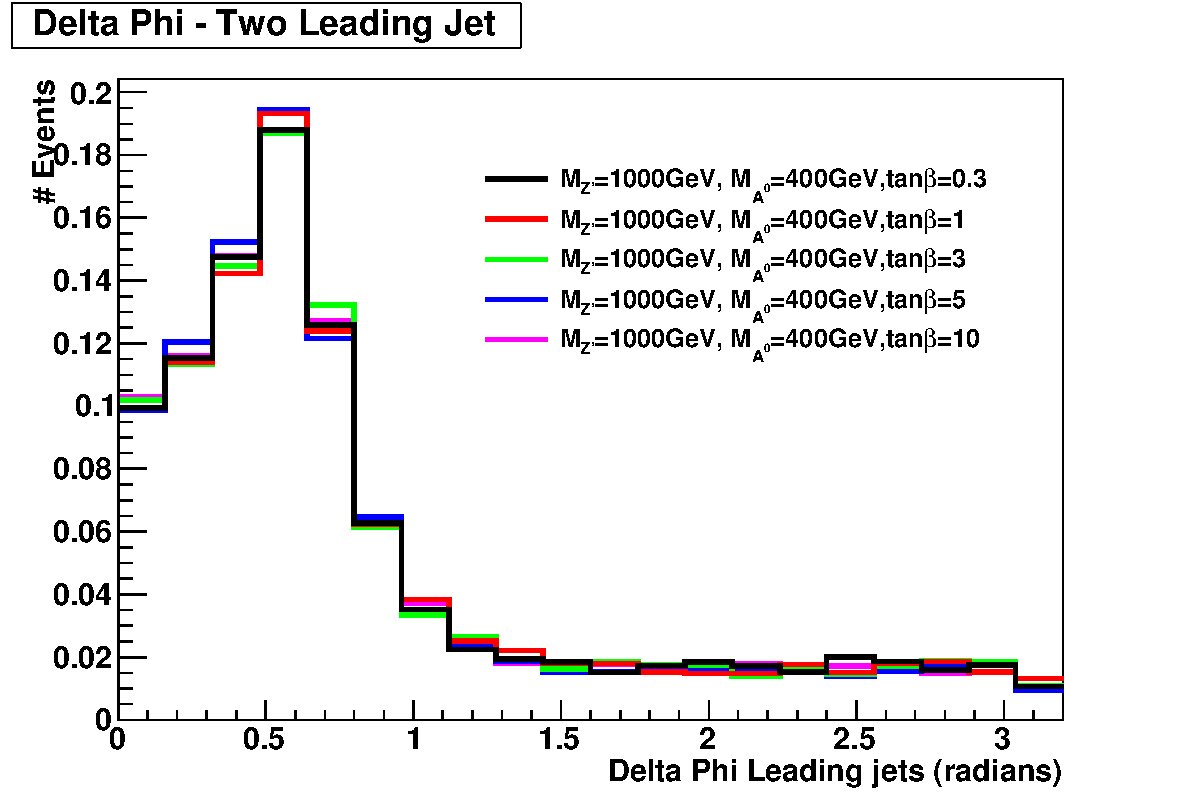
\includegraphics[width=0.60\linewidth]{figures/EW/monoH/2hdm/hxx_zp1000dm10gz01_dphi12}
}
\caption{Kinematic distributions of the signal process varying $\tan{\beta}$, in the case of a Higgs boson decaying into two $b$ quarks,
	after parameterized detector simulation: no kinematic dependence is observed on the mixing angle.}
\label{fig:DMH_tanbeta}
\end{figure}

Similarly, variations of $g_z$ do not lead to any kinematic changes. 
The value of $g_z$ for a given $M_{\Zprime}$ and $\tan \beta$ can be set according to the maximum value allowed by electroweak global 
fits and dijet constraints, as described in~\cite{Berlin:2014cfa}. Since this parameter does not influence the kinematics, 
we leave it up to individual analyses to decide whether they generate benchmark points only according to these external constraints.
%For \Zprime masses below $\sim 1.3$~\tev and larger $\tan \beta$, the $\rho_0$ constraint on $g_z$ is stronger than 
%dijet limits, while for $\tan \beta \lesssim 0.75$,
%the dijet constraints dominate even at low \Zprime masses. 

Since the DM pair are produced as a result of the decay of $A^0$, there are minimal kinematic changes when varying \mDM
as long as $\mDM<M_{A^0}/2$ so that $A^0$ production is on-shell, as shown in Fig.~\ref{fig:DMH_mdm} and~
\ref{fig:zprimeDecay} (before detector simulation). 

\begin{figure}[htpb!]
	\centering
	\subfloat[\MET distribution]{
		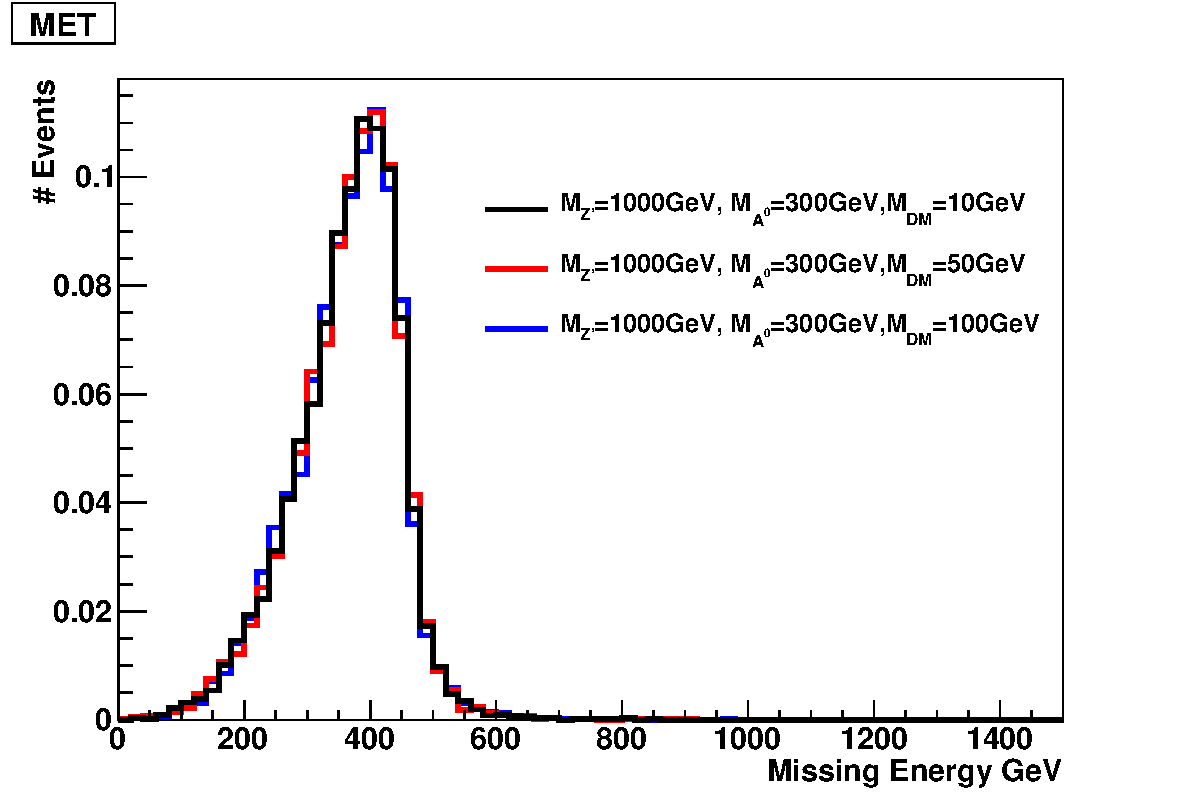
\includegraphics[width=0.60\linewidth]{figures/EW/monoH/2hdm/tanb1zp1000gz08_met}
	}
	\hfill
	\subfloat[$\Delta\phi$ distance between the two $b-$ jets]{
		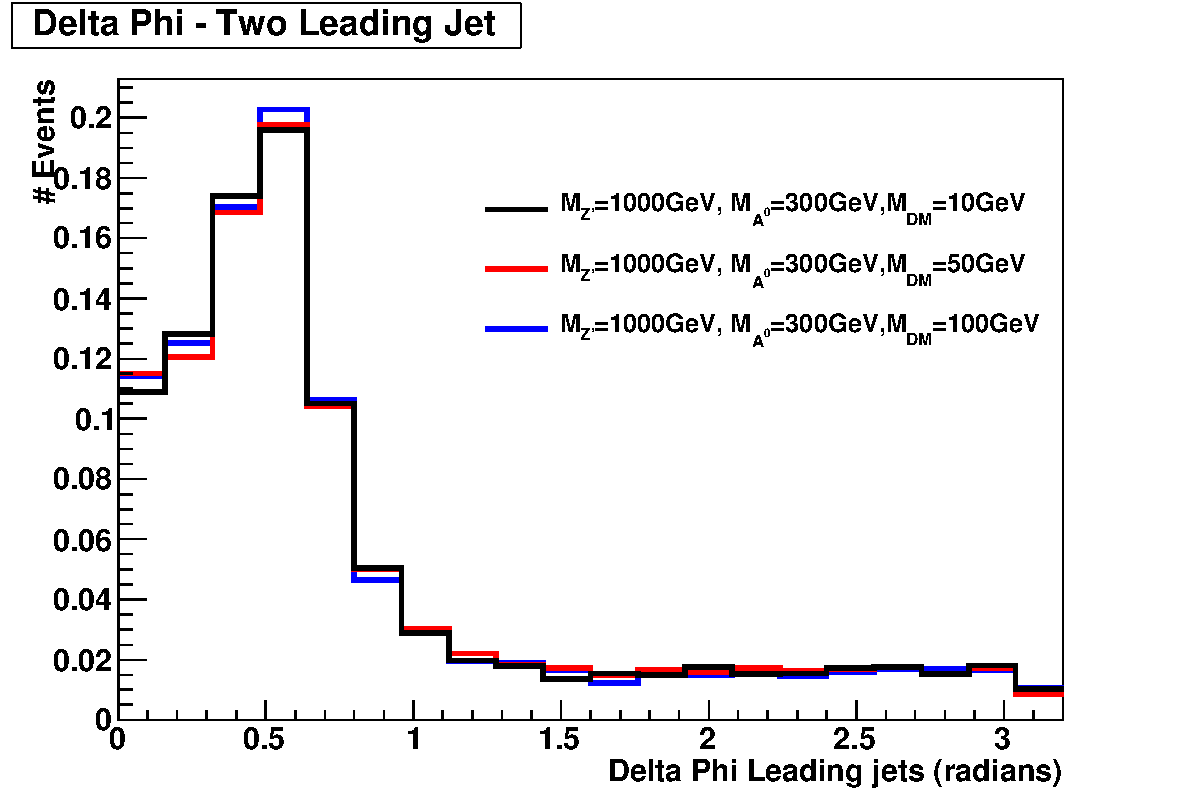
\includegraphics[width=0.60\linewidth]{figures/EW/monoH/2hdm/tanb1zp1000gz08_dphi12}
	}
	\caption{Kinematic distributions of the signal process varying \mDM: minimal kinematic dependency on \mDM as expected when $A^0$ is produced on-shell. Plots shown for $M_{\Zprime}=1000$~\gev, $M_{A^0}=300$~\gev.}
	\label{fig:DMH_mdm}
\end{figure}
 
  \begin{figure}[hbpt!]
  	\centering
  		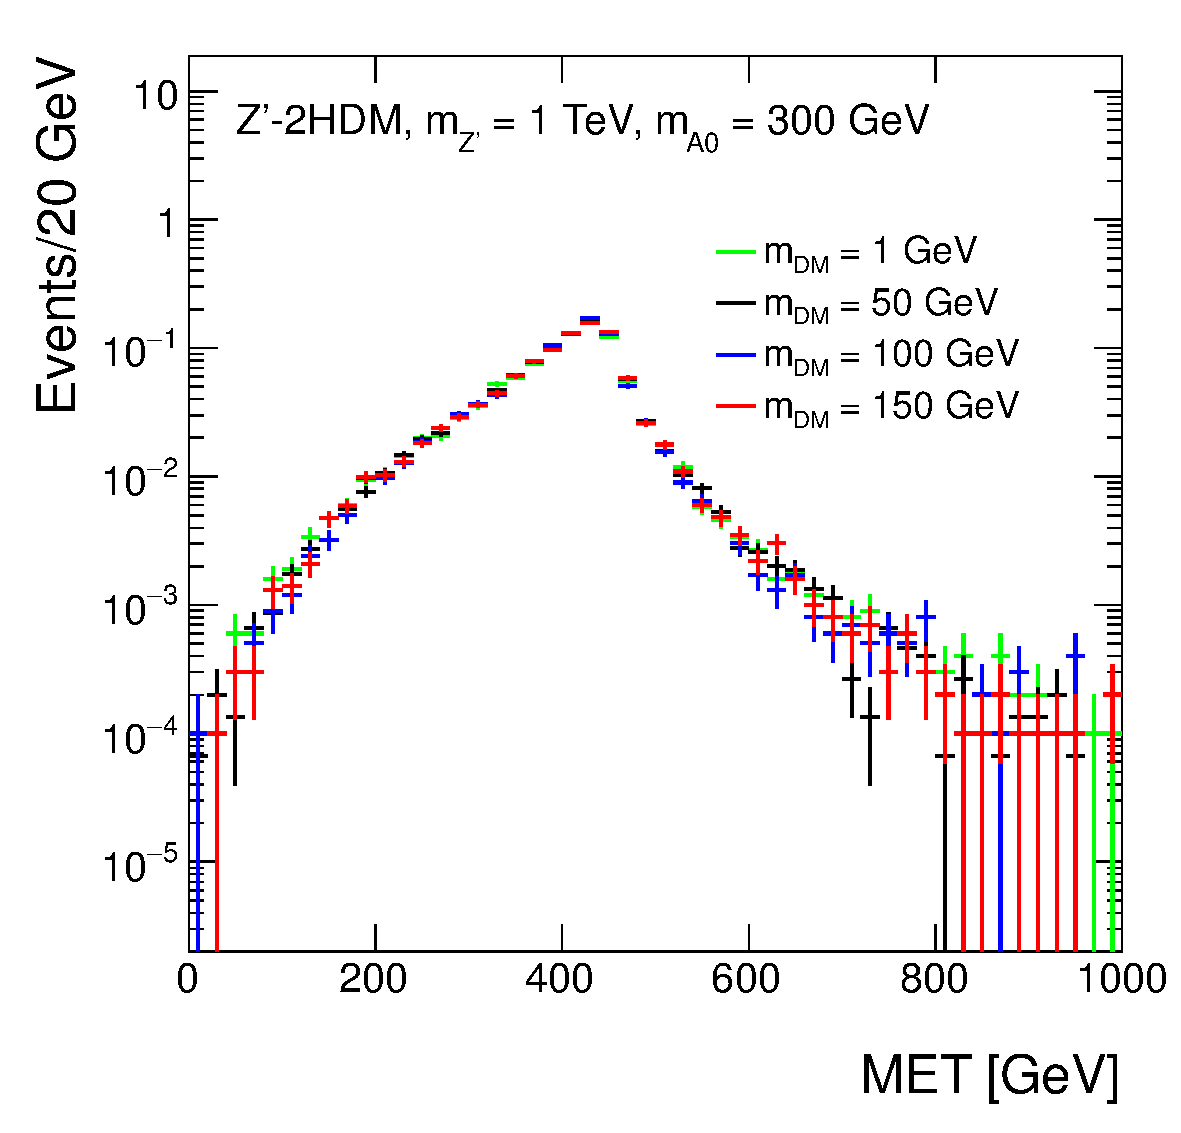
\includegraphics[width=0.60\linewidth]{figures/EW/monoH/zp2hdm_a0_300_MET_et_Log}
  		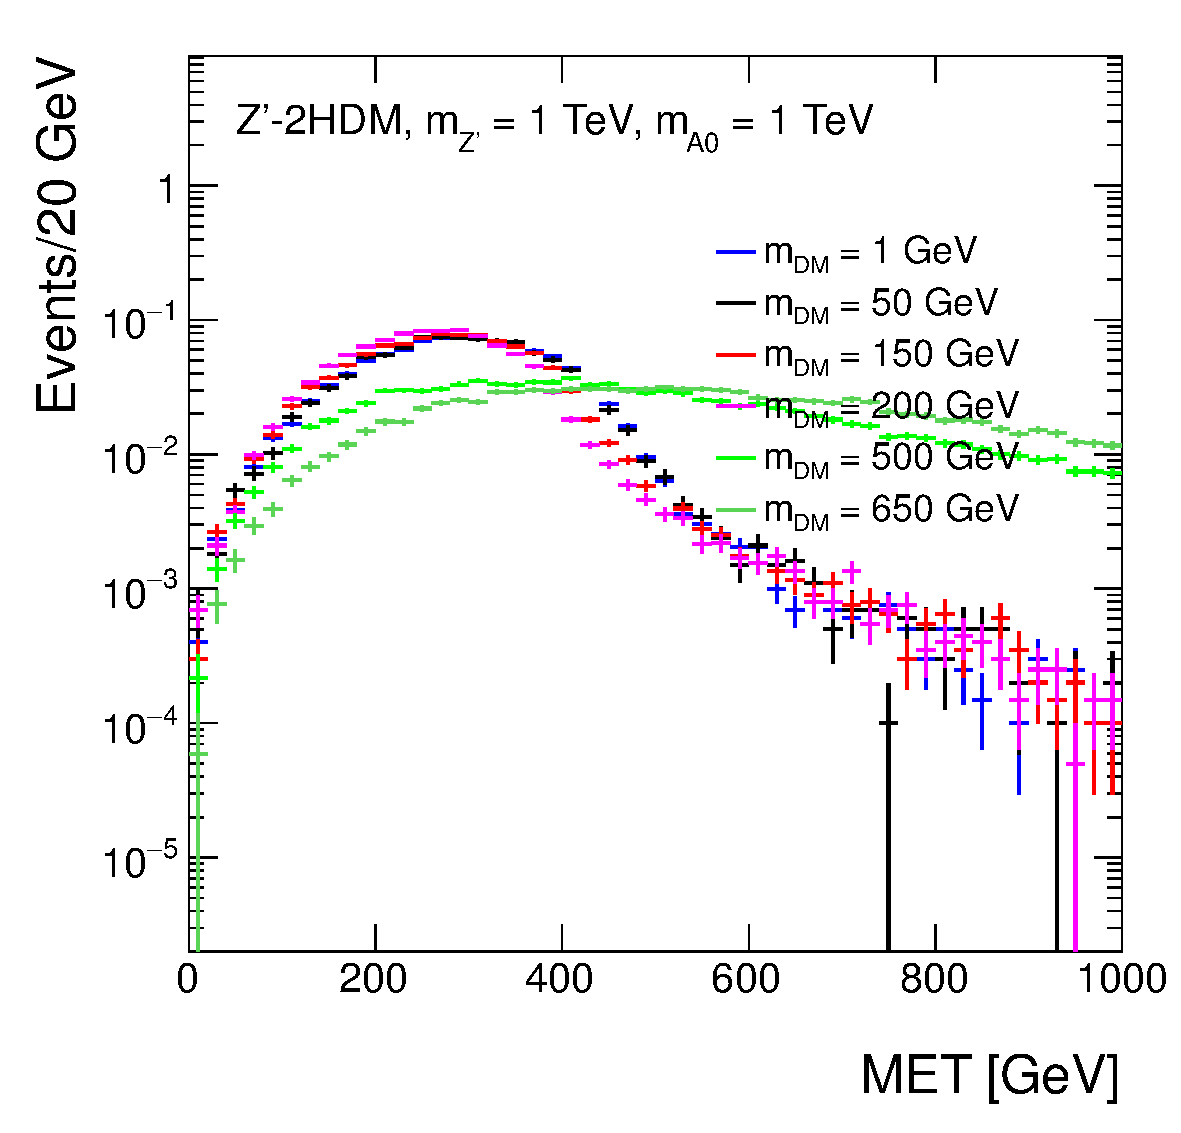
\includegraphics[width=0.60\linewidth]{figures/EW/monoH/zp2hdm_a0_1000_MET_et_Log}
  		\caption{Missing transverse momentum distributions at generator level in the \Zprime+2HDM 
  			scenario for different values of the DM mass \mDM, with 
  			$m_{\Zprime}$ = 1~\tev and $m_{A^0}$ = 300~\gev (left) and $m_{A^0}$ = 1~\tev (right).
  			\label{fig:zprimeDecay}}
  \end{figure}
  
We recommend to produce signal events for a fixed $g_z=0.8$, $\tan{\beta}=1$ and $\mDM=100$~\gev. For these values, we scan the 2-D parameter space of ${M_{\Zprime}, M_{A^0}}$ with $M_{\Zprime}$=600, 800, 1000, 1200, 1400~\gev, and $M_{A^0}$=300, 400, 500, 600, 700, 800~\gev with $M_{A^0} < M_{\Zprime}-m_h$, for a total of 24 points. The choice of scan is justified by the sensitivity study in~\cite{Berlin:2014cfa}: the expected LHC sensitivity for Run-2 is up to $M_{\Zprime} \sim 1.5$~\tev.
For the parameter scan, the DM mass is fixed to 100~\gev. For two $M_{\Zprime}$, $M_{A^0}$ value sets, we vary the DM mass to obtain sample cross section for rescaling results. 
All LO cross sections for the various parameter scan points are reported on HEPData ~\cite{HEPData}.
The parameter scan excludes the off-shell region, as the cross-sections are suppressed and the LHC would not have any
sensitivity to these benchmark points in early data. 

The kinematic distributions with varying $M_{\Zprime}$ for fixed $M_{A^0}$ are shown in Fig.~\ref{fig:DMH_mzp}, while the dependency on $M_{A^0}$ is shown in Fig.~\ref{fig:DMH_ma0}. 
  
 \begin{figure}[htpb!]
 	\centering
 	\subfloat[\MET distribution]{
 		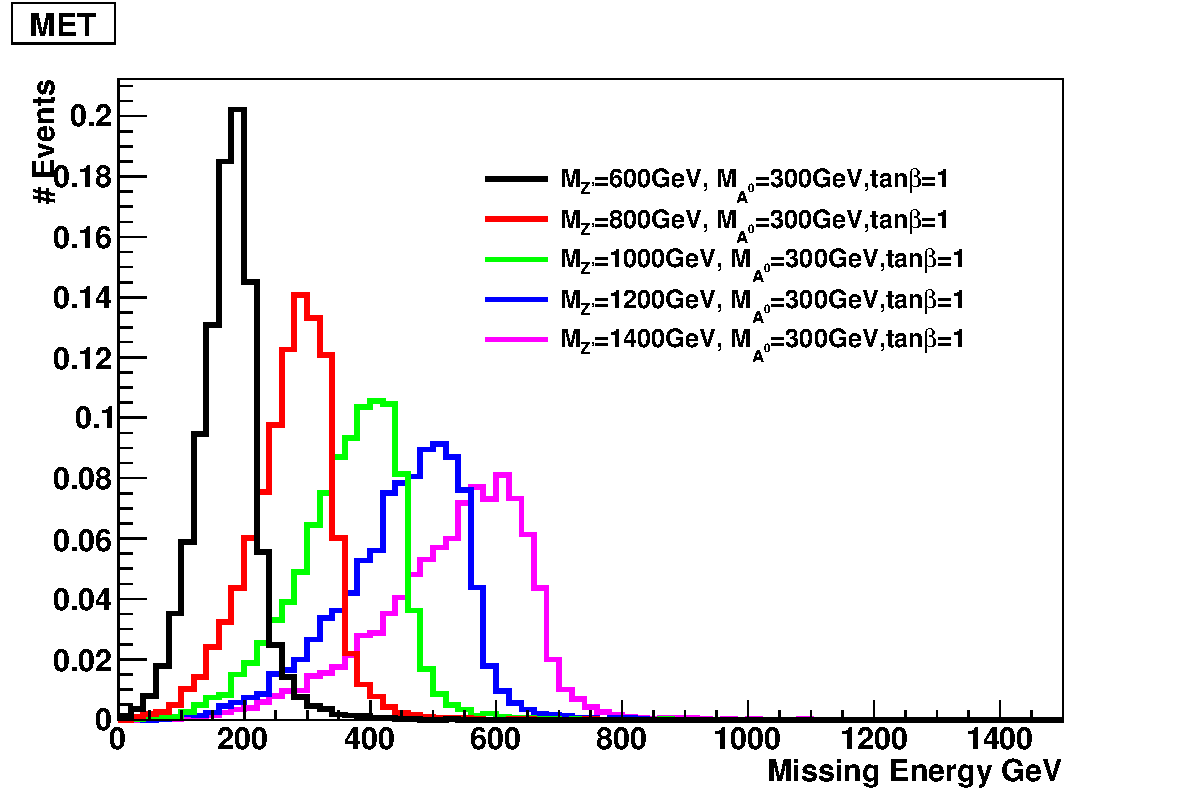
\includegraphics[width=0.60\linewidth]{figures/EW/monoH/2hdm/ZpA0h_tanb1gz08mA300mZp_met}
 	}
 	\hfill
 	\subfloat[Leading $b-$jet $p_T$  distribution]{
 		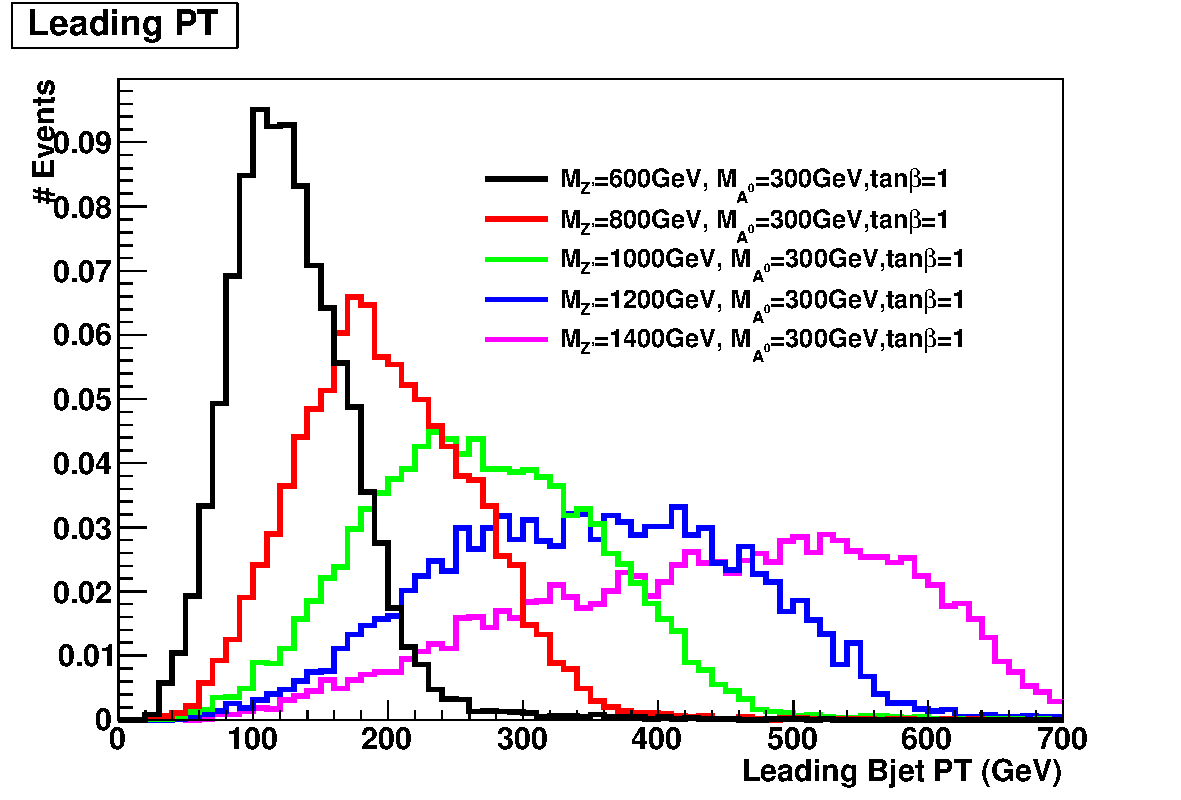
\includegraphics[width=0.60\linewidth]{figures/EW/monoH/2hdm/ZpA0h_tanb1gz08mA300mZp_p0}
 	}
 	\hfill
 	\subfloat[$\Delta\phi$ distance between the two $b-$ jets]{
 		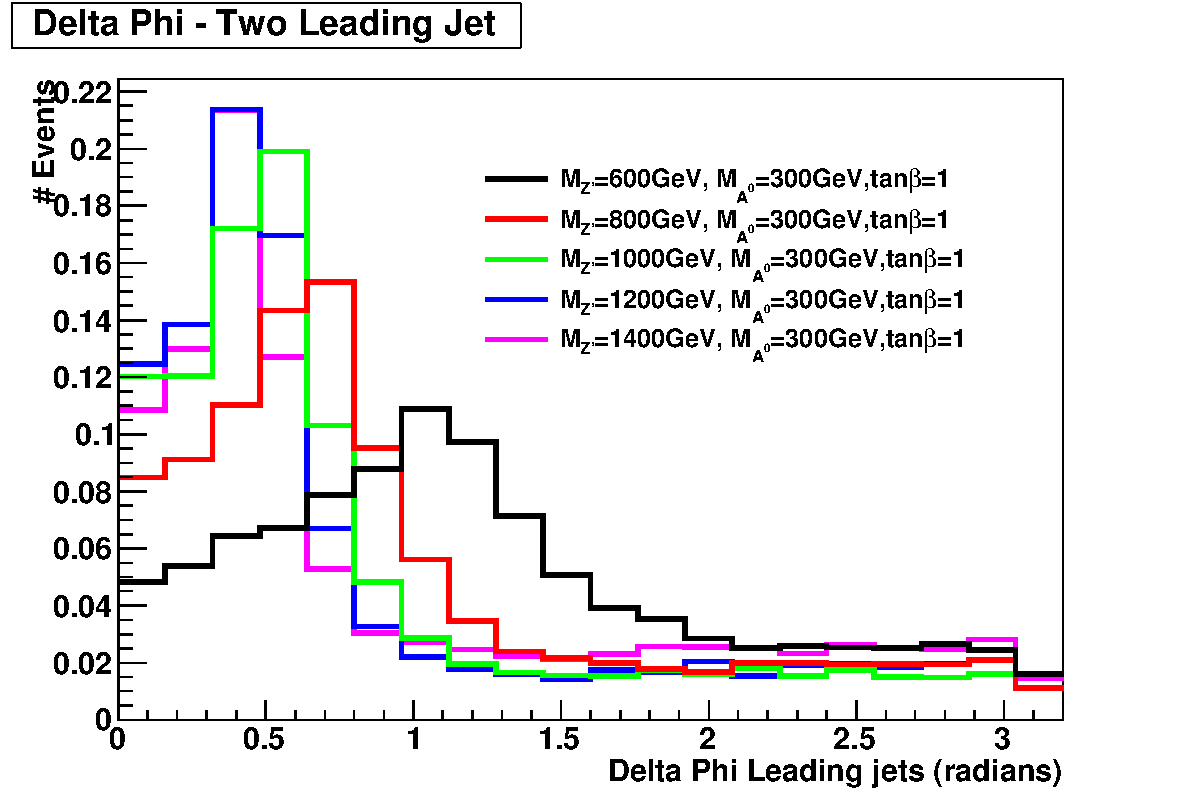
\includegraphics[width=0.60\linewidth]{figures/EW/monoH/2hdm/ZpA0h_tanb1gz08mA300mZp_dphi12}
 	}
 	
 	\caption{Kinematic distributions of the signal process varying $M_{\Zprime}$, for $\mDM=100$~\gev, $M_{A^0}=300$~\gev.}
 	\label{fig:DMH_mzp}
 \end{figure}
  
   \begin{figure}[htpb!]
   	\centering
   	\subfloat[\MET distribution]{
   		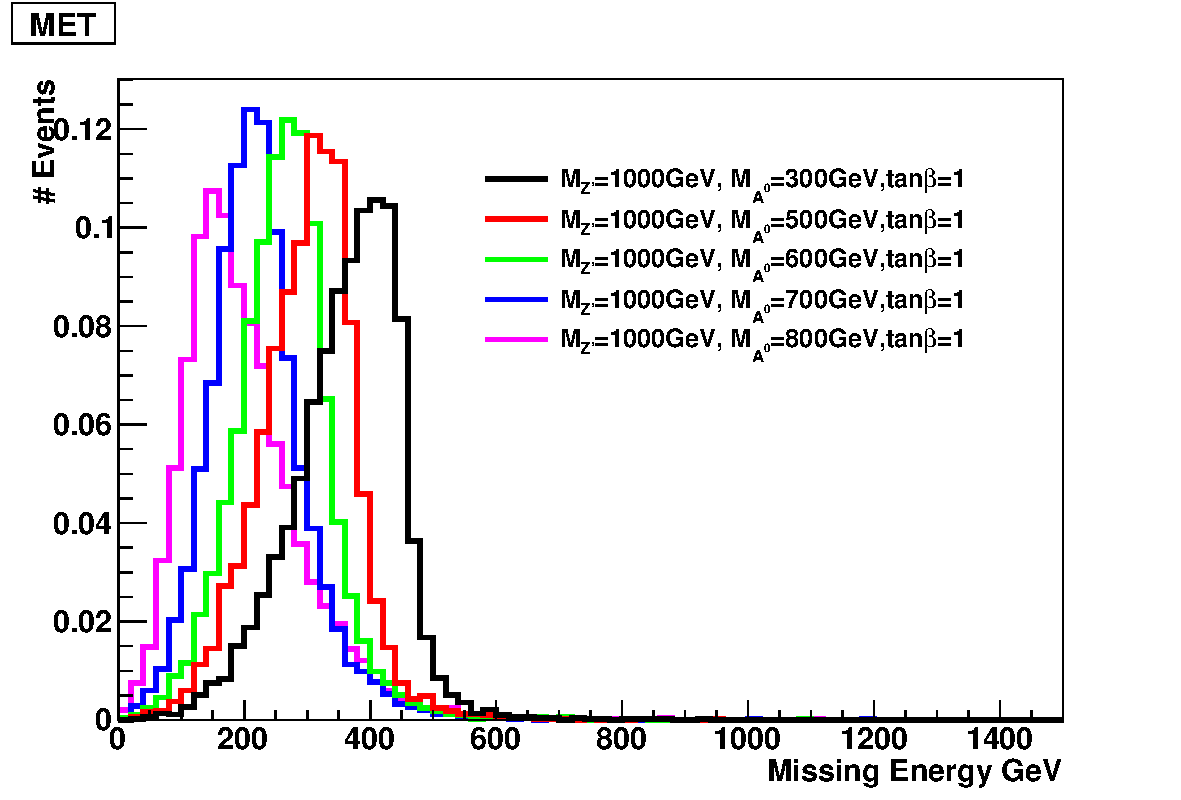
\includegraphics[width=0.60\linewidth]{figures/EW/monoH/2hdm/ZpA0h_tanb1gz08mZp1000mA_met}
   	}\hfill
   	\subfloat[Leading $b-$jet $p_T$ distribution]{
   		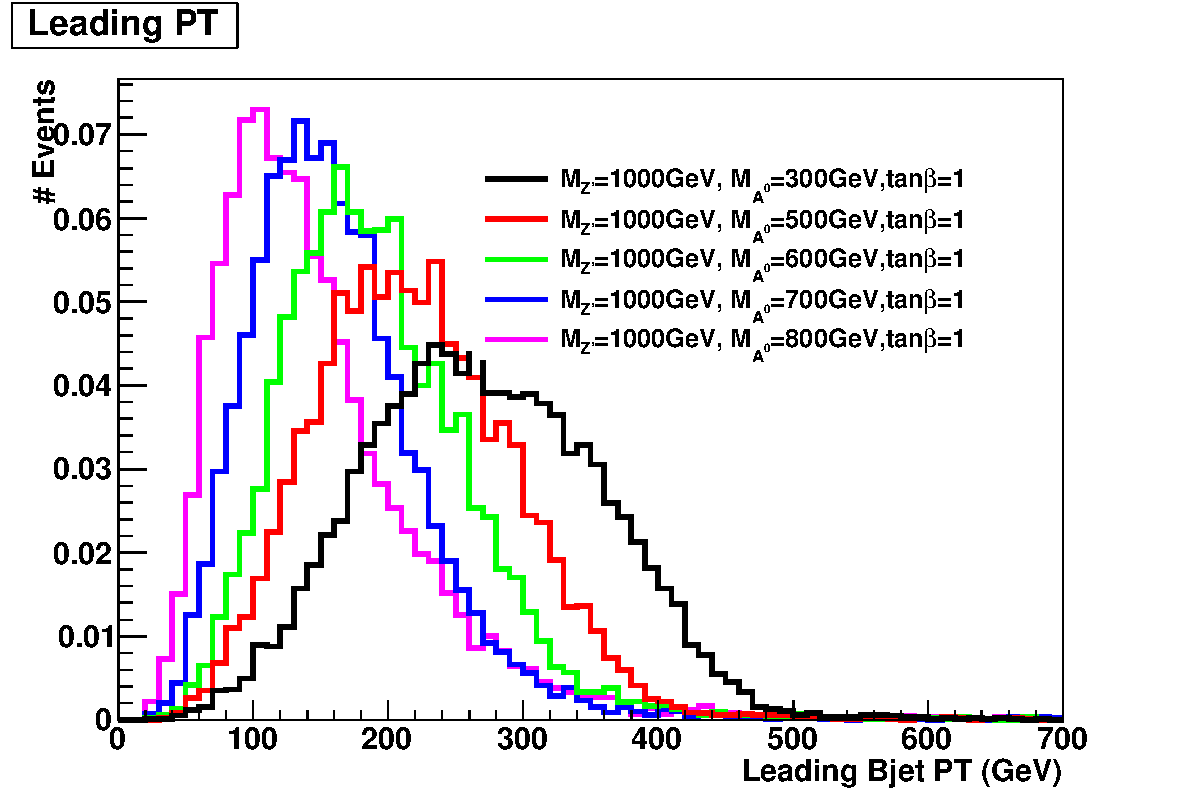
\includegraphics[width=0.60\linewidth]{figures/EW/monoH/2hdm/ZpA0h_tanb1gz08mZp1000mA_p0}
   	}
   	\hfill
   	\subfloat[$\Delta\phi$ distance between the two $b-$ jets]{
   		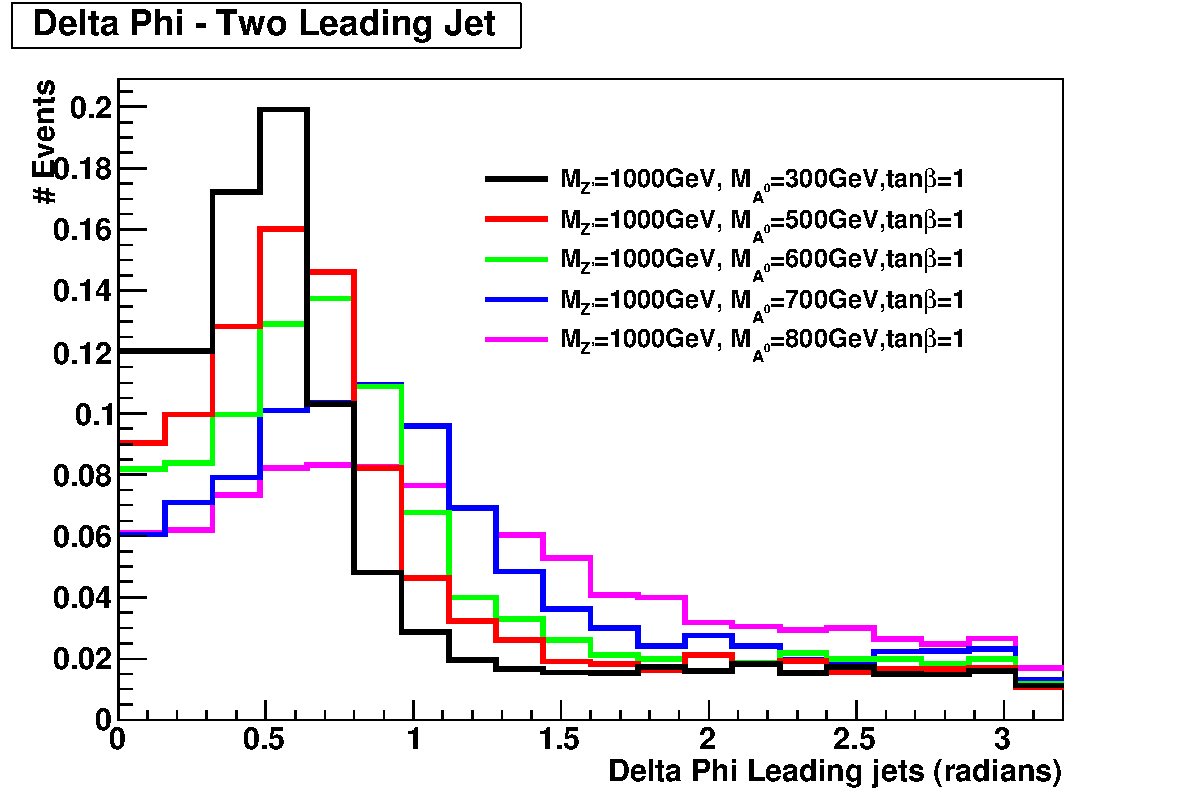
\includegraphics[width=0.60\linewidth]{figures/EW/monoH/2hdm/ZpA0h_tanb1gz08mZp1000mA_dphi12}
   	}
   	\caption{Kinematic distributions of the signal process varying $M_{A^0}$, for $\mDM=100$~\gev, $M_{\Zprime}=1000$~\gev.}
   	\label{fig:DMH_ma0}
   \end{figure}
      
 This model also allows for an additional source of Higgs plus \MET signal with a similar kinematics (Fig.~\ref{fig:DMH_zpincl}, shown with detector simulation 
 samples) to the signal process from the decay of $\Zprime \to h Z$, where the $Z$ decays invisibly. The partial decay width for the \Zprime is:

 \begin{equation}
 \Gamma_{\Zprime \to hZ}  = (g_z \cos \alpha \sin \beta)^2 \frac{|p|}{24 \pi} \left( \frac{ |p|^2 }{M_{\Zprime}^2} + 3 \frac{M_Z^2}{M_{\Zprime}^2} \right).
 \end{equation}
The values for the \Zprime masses scanned for those samples should follow those of the previous samples, 
namely values of $M_{\Zprime}=600, 800, 1000, 1200, 1400$~\gev.  This signal process has no $M_A$ dependence.
 
\begin{figure}[htpb!]
  	\centering
  	\subfloat[\MET distribution]{
  		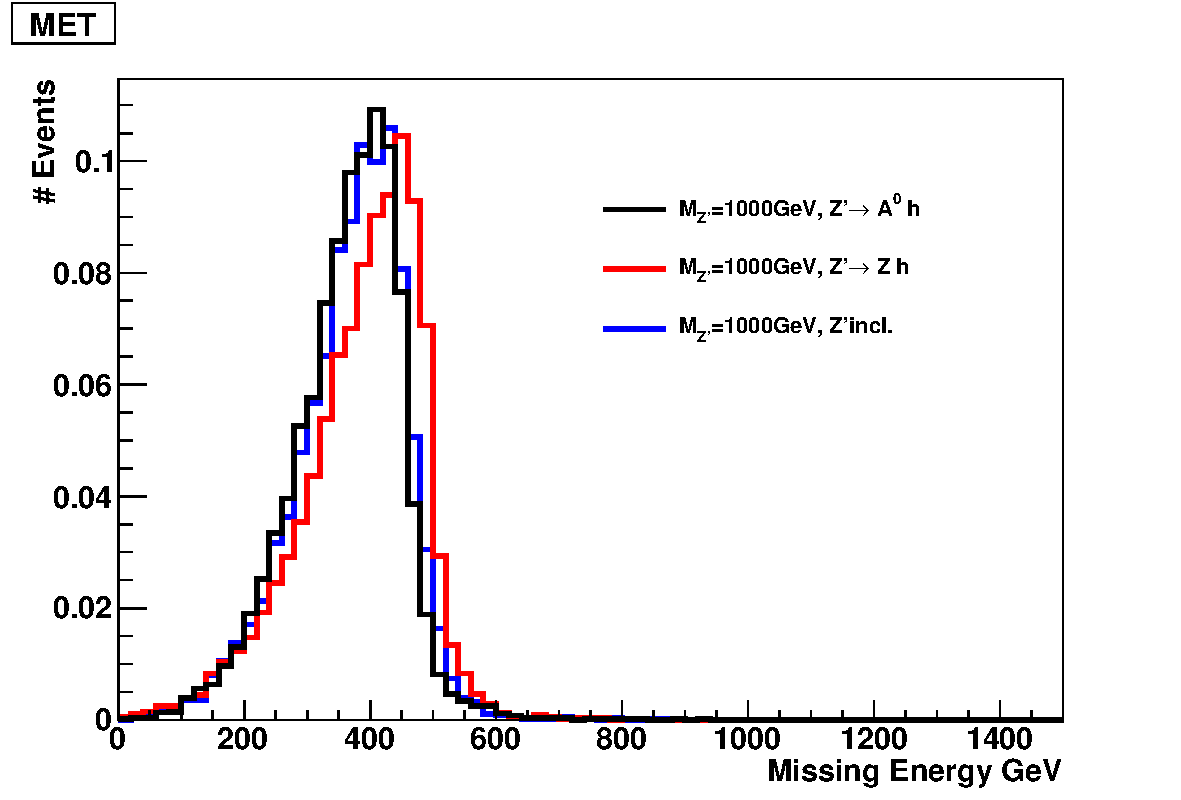
\includegraphics[width=0.60\linewidth]{figures/EW/monoH/2hdm/Zp_tanb1gz08mA300mZp1000_met}
  	}\hfill
  	\subfloat[Leading $b-$jet $p_T$ distribution]{
  		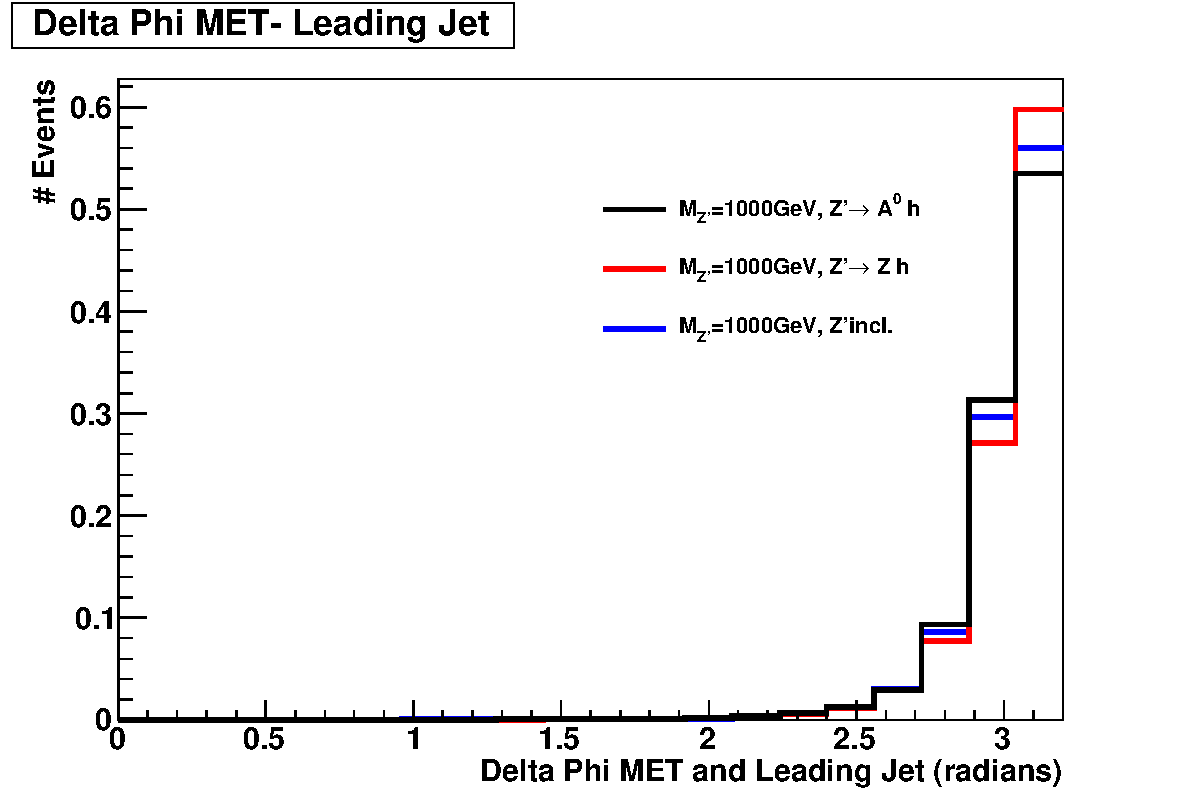
\includegraphics[width=0.60\linewidth]{figures/EW/monoH/2hdm/Zp_tanb1gz08mA300mZp1000_dphimetj0}
  	}
  	\hfill
  	\subfloat[$\Delta\phi$ distance between the two $b-$ jets]{
  		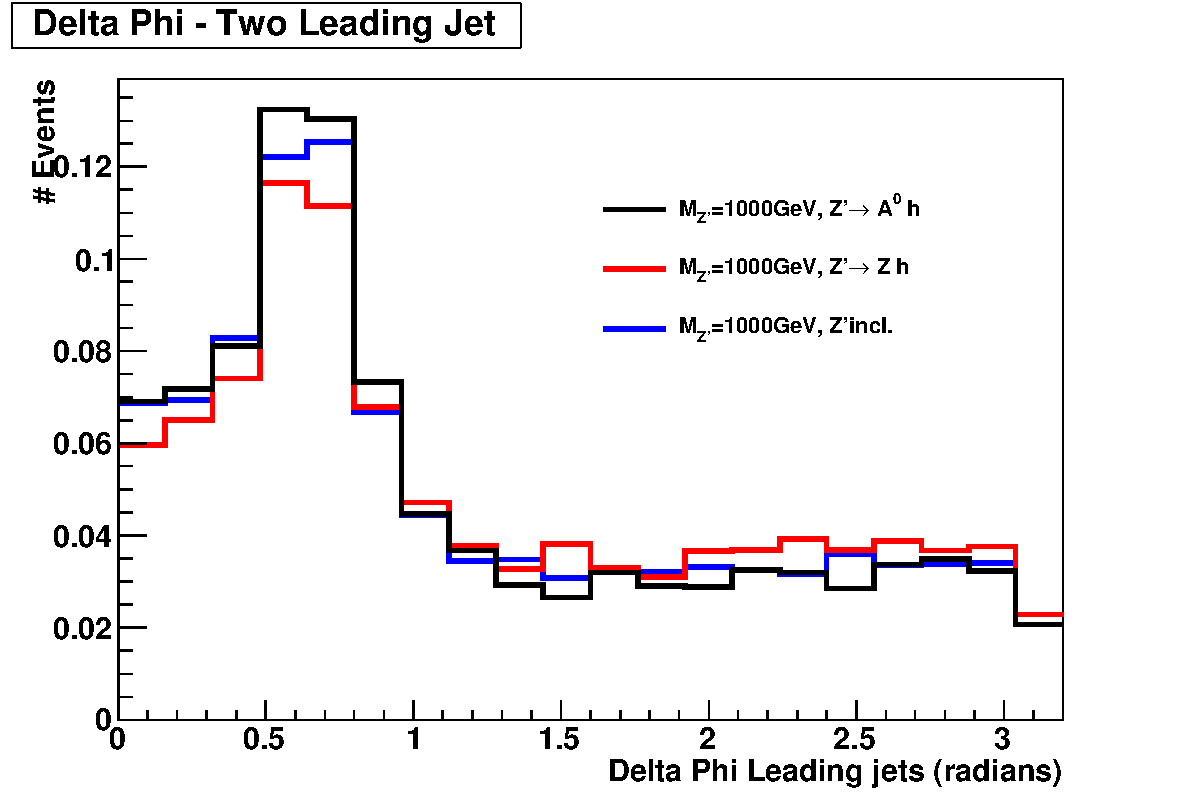
\includegraphics[width=0.60\linewidth]{figures/EW/monoH/2hdm/Zp_tanb1gz08mA300mZp1000_dphi12}
  	}
  	\caption{Kinematic distributions of $\Zprime \to A^0\,h$ exclusive production, $\Zprime \to Zh$ exclusive production and \Zprime inclusive production for $M_{\Zprime}=1000$~\gev and $M_{A^0}=300$~\gev}
  	\label{fig:DMH_zpincl}
\end{figure}



  
